\documentclass[9pt,twocolumn,a4paper]{extarticle}

\usepackage{amsmath}
\usepackage{fontspec}
\usepackage{unicode-math}
\setmainfont{CharisSIL-Regular.ttf}[BoldFont=CharisSIL-Bold.ttf,ItalicFont=CharisSIL-Italic.ttf,BoldItalicFont=CharisSIL-BoldItalic.ttf]
\setmathfont{STIXTwoMath-Regular.otf}
\setmonofont{consola.ttf}[BoldFont=consolab.ttf,ItalicFont=consolai.ttf,Scale=0.9]
\usepackage[top=1.5cm,bottom=2.3cm,left=1.35cm,right=1.35cm,columnsep=0.75cm,footskip=0.9cm,headsep=0.45cm]{geometry}
\usepackage{graphicx}
\usepackage{booktabs}
\usepackage{array}
\usepackage{xcolor}
\usepackage{titlesec}
\usepackage{caption}
\usepackage{float}
\usepackage{xtab}
\usepackage{listings}
\usepackage{fancyvrb}
\usepackage{tikz}
\usetikzlibrary{arrows.meta,positioning}
\tikzset{
  pbox/.style={draw=linkblue,thick,rounded corners=2pt,fill=linkblue!8,align=center,
               minimum height=9mm,text width=21mm,font=\footnotesize},
  pmine/.style={pbox,fill=linkblue!25,very thick},
  parr/.style={-{Stealth[length=2mm]},thick},
  plab/.style={font=\scriptsize,midway,fill=white,inner sep=1pt}}
\usepackage{fancyhdr}
\usepackage{setspace}
\usepackage{microtype}

\definecolor{linkblue}{RGB}{0,106,150}
\definecolor{bannergray}{RGB}{229,229,229}
\usepackage[colorlinks=true,linkcolor=linkblue,citecolor=linkblue,urlcolor=linkblue]{hyperref}

\titleformat{\section}{\normalsize\bfseries}{\thesection.}{0.55em}{}
\titleformat{\subsection}{\small\itshape}{\thesubsection.}{0.55em}{}
\titlespacing*{\section}{0pt}{10pt}{4pt}
\titlespacing*{\subsection}{0pt}{7pt}{3pt}
\setlength{\parskip}{0pt}
\setlength{\parindent}{1.1em}
\setlength{\arraycolsep}{2pt}
\setlength{\abovedisplayskip}{4pt}
\setlength{\belowdisplayskip}{4pt}
\renewcommand{\figurename}{Fig.}
\renewcommand{\tablename}{Table}
\renewcommand{\refname}{References}
\captionsetup{font={footnotesize},labelfont=bf,labelsep=period,justification=justified,singlelinecheck=false,skip=3pt}
\captionsetup[table]{position=top}
\emergencystretch=3em
\setlength{\textfloatsep}{9pt plus 2pt minus 2pt}
\setlength{\floatsep}{7pt plus 2pt minus 2pt}
\setlength{\intextsep}{7pt plus 2pt minus 2pt}
\linespread{1.04}
\raggedbottom

\lstset{basicstyle=\ttfamily\fontsize{7.2}{8.4}\selectfont,breaklines=true,breakindent=1.5em,breakautoindent=true,postbreak={\mbox{\textcolor{gray}{$\hookrightarrow$}\space}},frame=single,
  rulecolor=\color{gray!55},backgroundcolor=\color{gray!5},xleftmargin=2pt,xrightmargin=2pt,
  framesep=2pt,aboveskip=1pt,belowskip=3pt,columns=fullflexible,keepspaces=true}
\renewcommand{\lstlistingname}{Listing}
\lstdefinelanguage{GLSL}{sensitive=true,comment=[l]{//},
  morekeywords={uniform,in,out,flat,layout,void,if,else,for,return,discard}}
\lstset{numbers=none,keywordstyle=\bfseries,commentstyle=\itshape,
  showstringspaces=false,captionpos=t,frame=tb,rulecolor=\color{black},backgroundcolor=\color{white},
  framerule=0.5pt,aboveskip=0pt,belowskip=0pt,xleftmargin=1pt,xrightmargin=1pt,framexleftmargin=3pt,
  framexrightmargin=2pt,breaklines=true,breakindent=0pt,tabsize=2}
\captionsetup[lstlisting]{skip=2pt,font={footnotesize}}
\newenvironment{codebox}{\par\vspace{5pt}\noindent\begin{minipage}{\columnwidth}\hrule height 0.8pt\vspace{2pt}}{\end{minipage}\par\vspace{5pt}\noindent\ignorespaces}

\newcommand{\code}[1]{\texttt{#1}}
\newcommand{\Sig}{\symbf{\Sigma}}
\newcommand{\loc}[1]{\par\raggedright\noindent{\scriptsize\textit{#1}}\par\vspace{-1pt}}
\newcommand{\src}[1]{\par\raggedright\noindent{\footnotesize\textit{Source code:} \texttt{#1}}\par}
\newcommand{\spaced}[1]{\textls[160]{#1}}

\newcommand{\runauthor}{\textit{L.\,A.\ Kiet}}
\newcommand{\runtitle}{\textit{Splat Editor: a 3D Gaussian Splatting viewer and editor}}
\pagestyle{fancy}
\fancyhf{}
\renewcommand{\headrulewidth}{0pt}
\fancyhead[L]{\footnotesize\runauthor}
\fancyhead[R]{\footnotesize\runtitle}
\fancyfoot[C]{\footnotesize\thepage}
\fancypagestyle{first}{%
  \fancyhf{}\renewcommand{\headrulewidth}{0pt}%
}

\makeatletter
\renewcommand\@biblabel[1]{\textcolor{linkblue}{[#1]}}
\makeatother

\begin{document}
\thispagestyle{first}

\twocolumn[{%
\begin{@twocolumnfalse}
\vspace{-0.3cm}

{\fontsize{16.5}{20}\selectfont Splat Editor: a Viewer and Editor for\\3D Gaussian Splatting Scenes\par}
\vspace{0.4cm}
{\large Lê Anh Kiệt\textsuperscript{\,a}\par}
\vspace{0.2cm}
{\scriptsize\textsuperscript{a}\,\textit{International University, Vietnam National University Ho Chi Minh City, Vietnam} \quad Student ID: ITCSIU24047\par}
\vspace{0.3cm}
\noindent\rule{\textwidth}{0.4pt}
\vspace{0.25cm}

\noindent\begin{minipage}[t]{0.255\textwidth}
{\footnotesize\spaced{P R O J E C T \ \ I N F O}\par}
\vspace{2pt}\noindent\rule{\linewidth}{0.4pt}\par\vspace{3pt}
\textit{Keywords:}\\
3D Gaussian Splatting\\
Camera and projection\\
Lighting and shadows\\
Physics simulation\\
ImGui interface\par
\end{minipage}\hfill
\begin{minipage}[t]{0.715\textwidth}
{\footnotesize\spaced{A B S T R A C T}\par}
\vspace{2pt}\noindent\rule{\linewidth}{0.4pt}\par\vspace{3pt}
{\scriptsize\setlength{\parindent}{0pt}\linespread{1.08}\selectfont
This project builds Splat Editor, a program to view and edit 3D Gaussian Splatting (3DGS) scenes in Python and OpenGL~3.3. The program implements the 3DGS rendering pipeline itself: it reads the PLY file, projects ellipsoids to ellipses, sorts by depth and blends with alpha. On top of this, the project uses the six technique groups of the course: transformations, camera, texture, lighting, animation and interaction. The user can select, delete, undo and save the file.\par}
\end{minipage}

\vspace{0.25cm}
\noindent\rule{\textwidth}{0.4pt}
\vspace{0.35cm}
\end{@twocolumnfalse}
}]

%====================================================================
\section{Introduction and gaussian theory}
\label{chap:theory}
%====================================================================

\subsection{Introduction}
3D Gaussian Splatting (3DGS) shows a 3D scene with millions of soft ellipsoids, called gaussians \cite{kerbl2023gaussian}. The scene is trained from photos taken around an object (Fig.~\ref{fig:pipeline}). The resulting \code{.ply} file always has floating gaussians. So we need a program to view and clean the file. SuperSplat \cite{supersplat} does this in the browser. I wrote a similar editor in Python and OpenGL~3.3.

\begin{figure}[H]
\centering
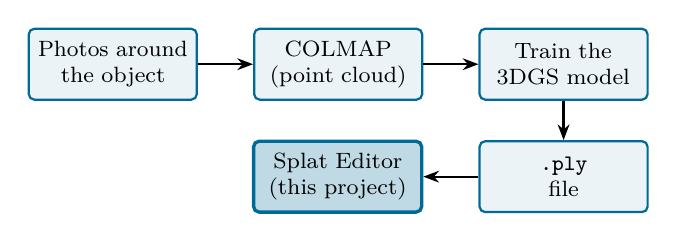
\begin{tikzpicture}[
  node distance=5mm and 7mm,
  box/.style={draw=linkblue,thick,rounded corners=2pt,fill=linkblue!8,align=center,
              minimum height=9mm,text width=19mm,font=\footnotesize},
  mine/.style={box,fill=linkblue!25,very thick},
  arr/.style={-{Stealth[length=2mm]},thick}]
  \node[box] (photos) {Photos around\\the object};
  \node[box,right=of photos] (colmap) {COLMAP\\(point cloud)};
  \node[box,right=of colmap] (train) {Train the\\3DGS model};
  \node[box,below=of train] (ply) {\code{.ply}\\file};
  \node[mine,left=of ply] (editor) {Splat Editor\\(this project)};
  \draw[arr] (photos) -- (colmap);
  \draw[arr] (colmap) -- (train);
  \draw[arr] (train) -- (ply);
  \draw[arr] (ply) -- (editor);
\end{tikzpicture}
\caption{The workflow from photos to Splat Editor. COLMAP \cite{schonberger2016colmap} finds the camera positions.}
\label{fig:pipeline}
\end{figure}

The project has two parts. Part one is the 3DGS rendering pipeline, from the file to the shader. Part two is the six technique groups of the course (Table~\ref{tab:map}).

\begin{table}[H]
\centering
\caption{Technique groups and sections.}
\label{tab:map}
\footnotesize
\begin{tabular}{@{}lll@{}}
\toprule
Group & Main content & Section \\
\midrule
T1 & layers, matrix $\mathbf{M}$ & \ref{chap:t1} \\
T2 & view/projection matrices, EWA, blending, cameras & \ref{chap:t2} \\
T3 & character skin texture & \ref{chap:t3} \\
T4 & SH colour, Phong, shadow map & \ref{chap:t4} \\
T5 & day--night, collision, player & \ref{chap:t5} \\
T6 & selection brush, delete/undo, ImGui, HUD & \ref{chap:t6} \\
\bottomrule
\end{tabular}
\end{table}

\subsection{Program structure}
The source is split by role: \code{core} holds only data and math, so it does not depend on OpenGL; \code{render} holds all OpenGL calls and shaders; \code{ui} builds the interface; and \code{app.py} ties the parts together. Figure~\ref{fig:tree} lists representative files only.

\begin{figure}[H]
\centering
\begin{Verbatim}[fontsize=\fontsize{5.6}{6.6}\selectfont,frame=single]
SplatOpenGL/
|-- main.py              # entry point: python main.py [scene.ply]
|-- requirements.txt     # numpy, PyOpenGL, glfw, imgui-bundle
|-- report/              # LaTeX report
`-- splat_editor/
    |-- app.py           # main loop, ties everything together
    |-- core/            # data and math, no OpenGL
    |   |-- splats.py    # gaussian arrays
    |   |-- layer.py     # one PLY file + transform + selection
    |   |-- scene.py     # the set of layers
    |   |-- math3d.py    # matrices V, P, Euler angles, quaternions
    |   |-- lighting.py  # sun, lamps, day--night
    |   |-- physics.py   # voxel collision, jumping
    |   |-- avatar_pose.py  # character joint angles
    |   |-- lod.py       # level-of-detail selection
    |   `-- history.py   # undo
    |-- io/              # file reading / writing
    |   |-- ply.py       # read / write PLY
    |   `-- codec.py     # PLY columns <-> Splats
    |-- editor/          # editing
    |   |-- editor.py    # open, save, delete, select
    |   `-- brush.py     # brush selection
    |-- render/          # OpenGL
    |   |-- splat_renderer.py  # draws gaussians (2 passes)
    |   |-- sorter.py    # depth sort (background thread)
    |   |-- camera.py    # orbit / fly camera
    |   |-- avatar_renderer.py # draws the character
    |   |-- shader.py    # compiles GLSL
    |   |-- shaders/     # splat_prep.vert, splat.vert/.frag, ...
    |   `-- textures/    # skinzom.png
    `-- ui/              # ImGui interface
        |-- window.py    # GLFW window
        |-- input.py     # keyboard, mouse
        `-- sections.py  # control panels
\end{Verbatim}
\caption{Directory tree of the program (main files only).}
\label{fig:tree}
\end{figure}

\subsection{Input data}
\label{sec:input}
The input is a \code{.ply} file made by 3DGS training. Training starts from the COLMAP point cloud and puts one gaussian at each point. Then it repeats three steps. It renders the gaussians. It compares the image with the real photo. It updates the parameters of every gaussian. It also removes useless gaussians and splits gaussians that are too large.

The file has two parts: a text header and a binary body. The header lists the properties. The body has one record per gaussian. Every value is a 32-bit float. Table~\ref{tab:ply} lists the properties. With SH of degree 3, one record has 62 values, or 248 bytes. Fig.~\ref{fig:csv} shows the first rows of a file, exported as CSV.

\begin{table}[H]
\centering
\caption{Properties of one gaussian in the PLY file.}
\label{tab:ply}
\footnotesize
\begin{tabular}{@{}p{2.3cm}p{0.9cm}p{4.4cm}@{}}
\toprule
Property & Count & Meaning \\
\midrule
\code{x, y, z} & 3 & centre $\symbf{\mu}$ \\
\code{nx, ny, nz} & 3 & normal, always 0, not used \\
\code{f\_dc\_0..2} & 3 & base colour (SH degree 0) \\
\code{f\_rest\_*} & 45 & SH coefficients of degrees 1--3 \\
\code{opacity} & 1 & raw opacity \\
\code{scale\_0..2} & 3 & logarithm of the size \\
\code{rot\_0..3} & 4 & rotation quaternion \\
\bottomrule
\end{tabular}
\end{table}

\begin{figure}[H]
\centering
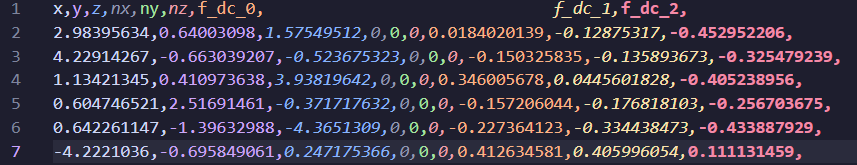
\includegraphics[width=\columnwidth]{figures/csv_head.png}\\[2pt]
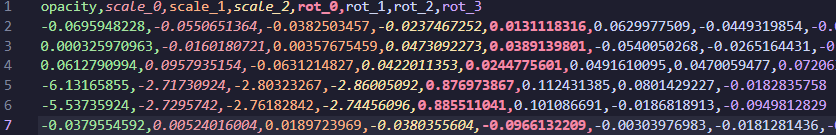
\includegraphics[width=\columnwidth]{figures/csv_tail.png}
\caption{The first six gaussians of a PLY file, shown as CSV. Top: position, normal and base colour. Bottom: opacity, scale and rotation. The \code{f\_rest} columns in between are hidden.}
\label{fig:csv}
\end{figure}

The program maps a binary file straight into memory. So a file with millions of gaussians opens almost at once. Fig.~\ref{fig:viewer} shows a small capture of a person. The blurry blobs around the body are the floating gaussians that the editor must remove. The main test scene is a street with about 5 million gaussians (Fig.~\ref{fig:scene}).

\begin{figure}[H]
\centering
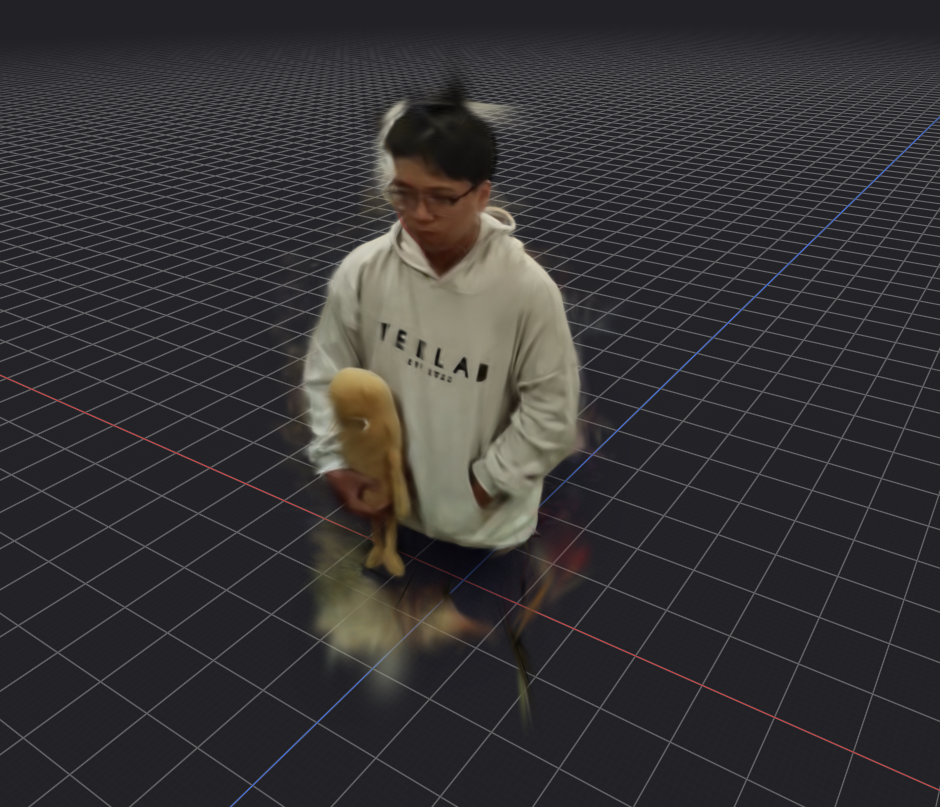
\includegraphics[width=0.6\columnwidth]{figures/viewer.png}
\caption{A PLY file of a captured person. Floating gaussians are visible around the body and near the ground.}
\label{fig:viewer}
\end{figure}

\begin{figure}[H]
\centering
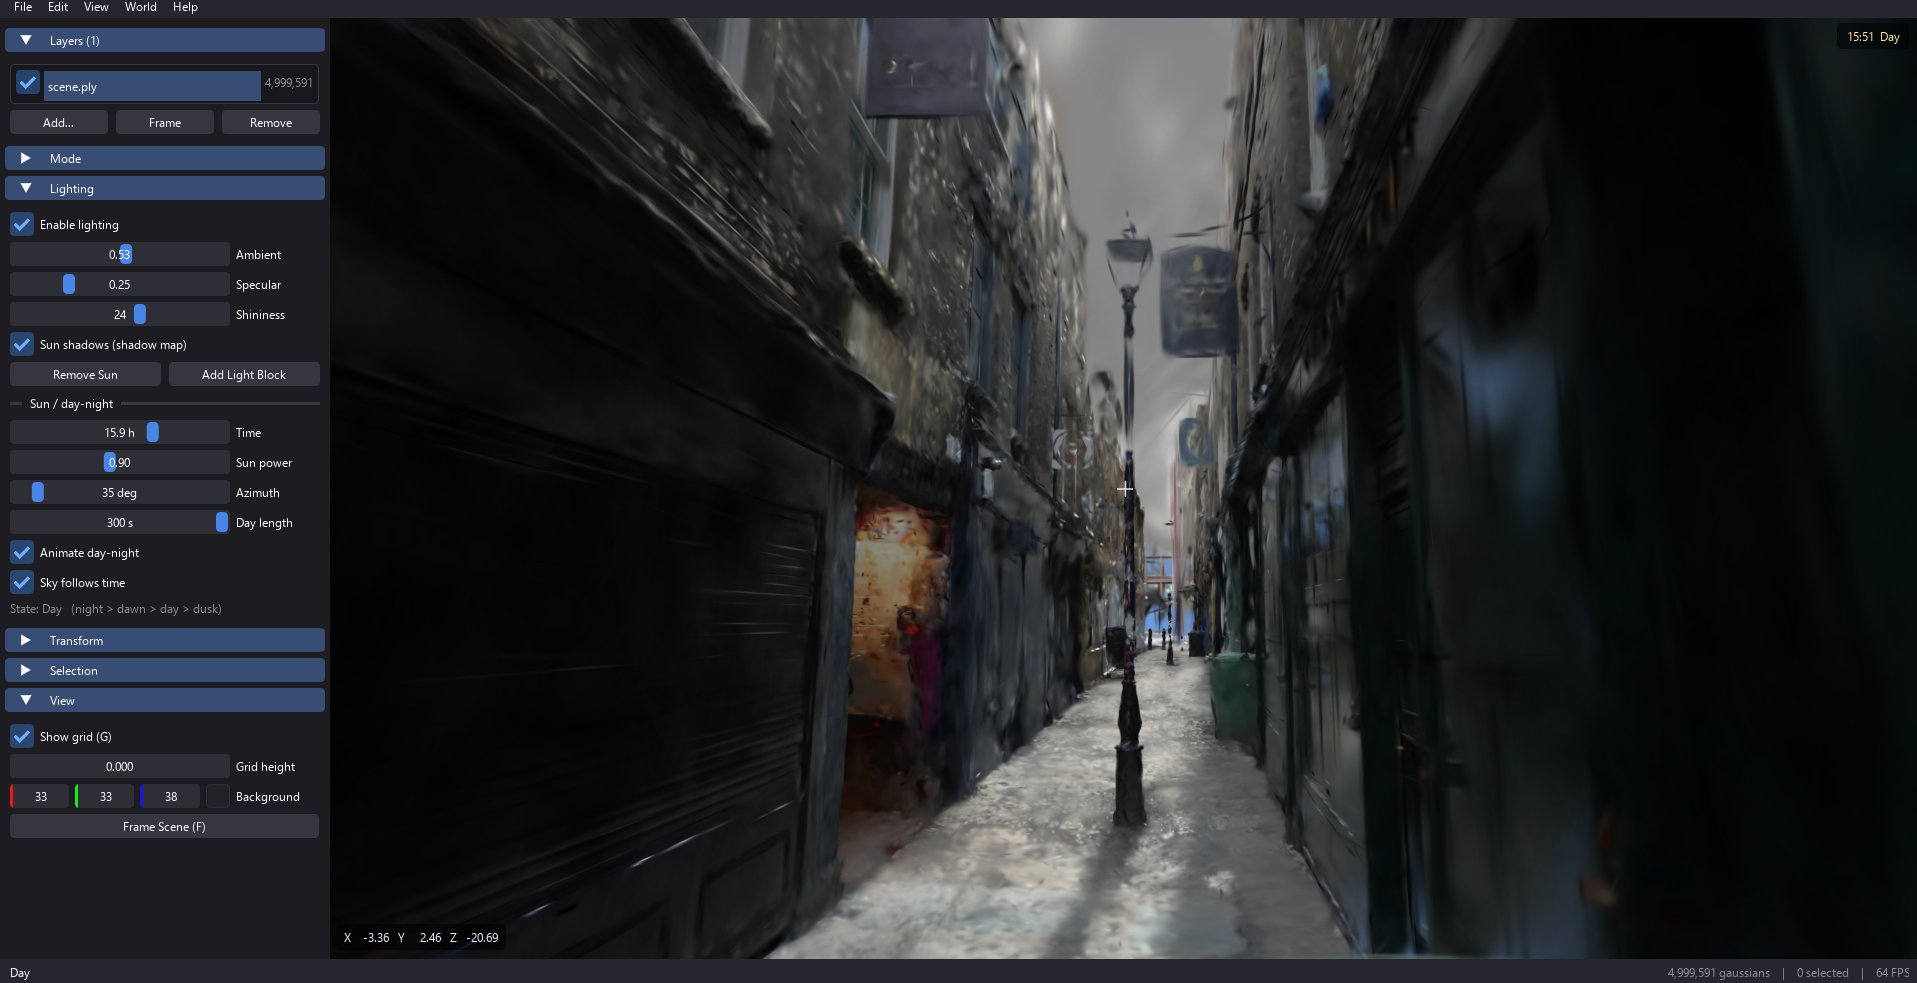
\includegraphics[width=\columnwidth]{figures/t4-day.png}\\[3pt]
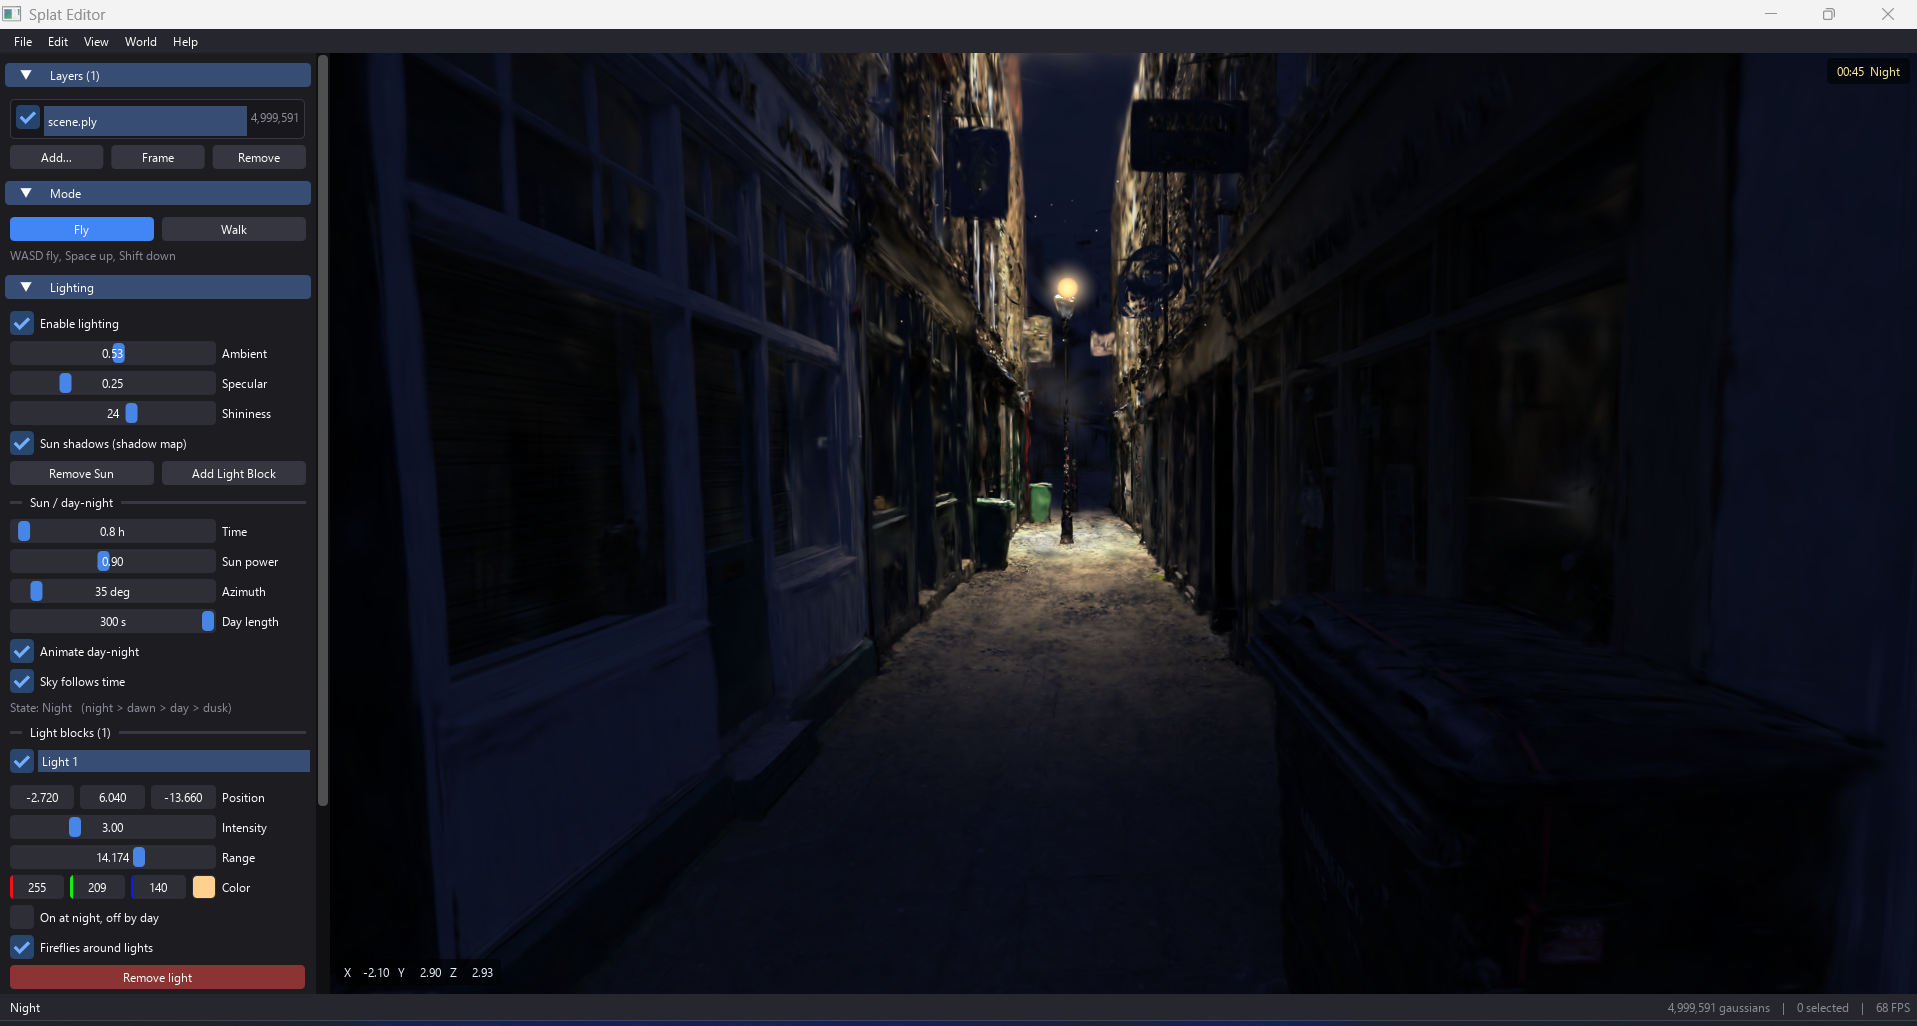
\includegraphics[width=\columnwidth]{figures/t4-night.png}
\caption{A scene of about 5 million gaussians in Splat Editor, by day (top) and by night (bottom).}
\label{fig:scene}
\end{figure}

\subsection{Gaussians and the PLY file}
\label{sec:decode}
Each gaussian has a position $\symbf{\mu}$, a colour $\mathbf{c}$, an opacity $\alpha$, a size $\mathbf{s}$ and a rotation $\symbf{q}$ (quaternion). Its density falls off smoothly from the centre. We can picture it as an ellipsoid (Fig.~\ref{fig:g2e}). The PLY file stores raw values. The program decodes them on load:
\begin{itemize}\itemsep0pt
  \item Size: $s_i=\exp(\code{scale\_i})$.
  \item Opacity: $\alpha=1/(1+e^{-\code{opacity}})$.
  \item Colour: $\mathrm{RGB}=0.5+C_0\,\code{f\_dc}$, with $C_0\approx0.2821$.
  \item Rotation: the quaternion \code{rot\_0..3} is normalised to length 1.
\end{itemize}
On save, the program does the reverse.

\begin{codebox}
\begin{lstlisting}[language=Python,caption={\code{io/codec.py}, \code{SplatCodec.decode}: decoding the raw PLY values},label={lst:decode}]
SH_C0 = 0.28209479177387814
colors = 0.5 + SH_C0 * np.stack([col('f_dc_0'), col('f_dc_1'), col('f_dc_2')], axis=1)
alphas = 1.0 / (1.0 + np.exp(-col('opacity')))
scales = np.exp(np.stack([col('scale_0'), col('scale_1'), col('scale_2')], axis=1))
q = np.stack([col('rot_0'), col('rot_1'), col('rot_2'), col('rot_3')], axis=1)
length = np.linalg.norm(q, axis=1, keepdims=True)
q = q / np.maximum(length, 1e-12)
\end{lstlisting}
\end{codebox}

\begin{figure}[H]
\centering
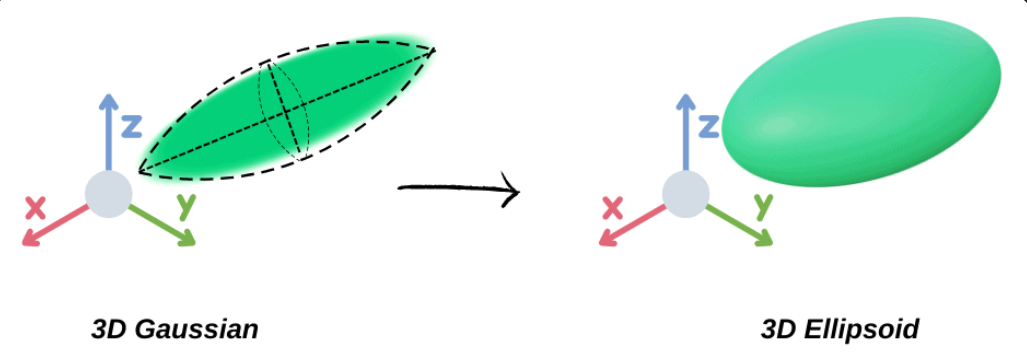
\includegraphics[width=\columnwidth]{figures/1 (4).png}
\caption{A 3D gaussian is a soft blob. Its surface at one standard deviation is an ellipsoid.}
\label{fig:g2e}
\end{figure}

The shape of a gaussian is stored in its covariance matrix $\Sig$. It is built from the scale matrix $\mathbf{S}=\mathrm{diag}(\mathbf{s})$ and the rotation matrix $\mathbf{R}(\symbf{q})$:
\begin{equation}
\Sig=\mathbf{R}\,\mathbf{S}\mathbf{S}^{\top}\mathbf{R}^{\top}.
\label{eq:cov3d}
\end{equation}
Fig.~\ref{fig:rs} gives the two matrices. Fig.~\ref{fig:ellipsoid} draws the result for the first gaussian of Fig.~\ref{fig:csv}. The three sizes $s_0,s_1,s_2$ are the semi-axes of the ellipsoid. The quaternion turns these axes in space. Section~\ref{sec:ewa} projects this ellipsoid to the screen.

\begin{codebox}
\begin{lstlisting}[language=GLSL,caption={\code{render/shaders/splat\_prep.vert}: building $\Sigma=\mathbf{R}\mathbf{S}\mathbf{S}^{\top}\mathbf{R}^{\top}$},label={lst:cov3d}]
vec3 scale = vec3(unpackHalf(t1.y), halfToFloat(t1.z & 65535u));
vec4 q = normalize((vec4(uvec4(t1.w, t1.w >> 8u, t1.w >> 16u, t1.w >> 24u)
                         & 255u) - 128.0) / 127.0);
float w = q.x, x = q.y, y = q.z, z = q.w;
mat3 R = mat3(1.0 - 2.0 * (y * y + z * z), 2.0 * (x * y + w * z), 2.0 * (x * z - w * y),
              2.0 * (x * y - w * z), 1.0 - 2.0 * (x * x + z * z), 2.0 * (y * z + w * x),
              2.0 * (x * z + w * y), 2.0 * (y * z - w * x), 1.0 - 2.0 * (x * x + y * y));
mat3 M = R * mat3(scale.x, 0.0, 0.0, 0.0, scale.y, 0.0, 0.0, 0.0, scale.z);
mat3 sigma = M * transpose(M);
\end{lstlisting}
\end{codebox}

\begin{figure}[H]
\centering
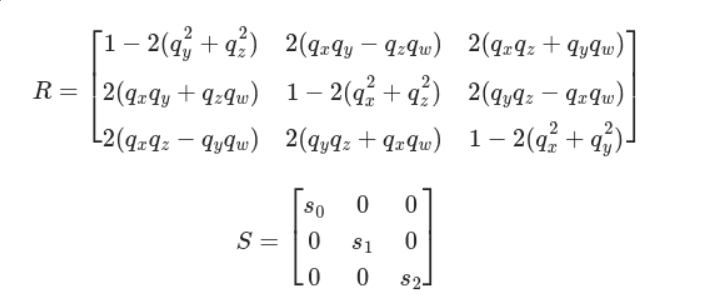
\includegraphics[width=0.75\columnwidth]{figures/1 (5).png}
\caption{The rotation matrix $\mathbf{R}$ from the quaternion $(q_w,q_x,q_y,q_z)$ and the scale matrix $\mathbf{S}$.}
\label{fig:rs}
\end{figure}

\begin{figure}[H]
\centering
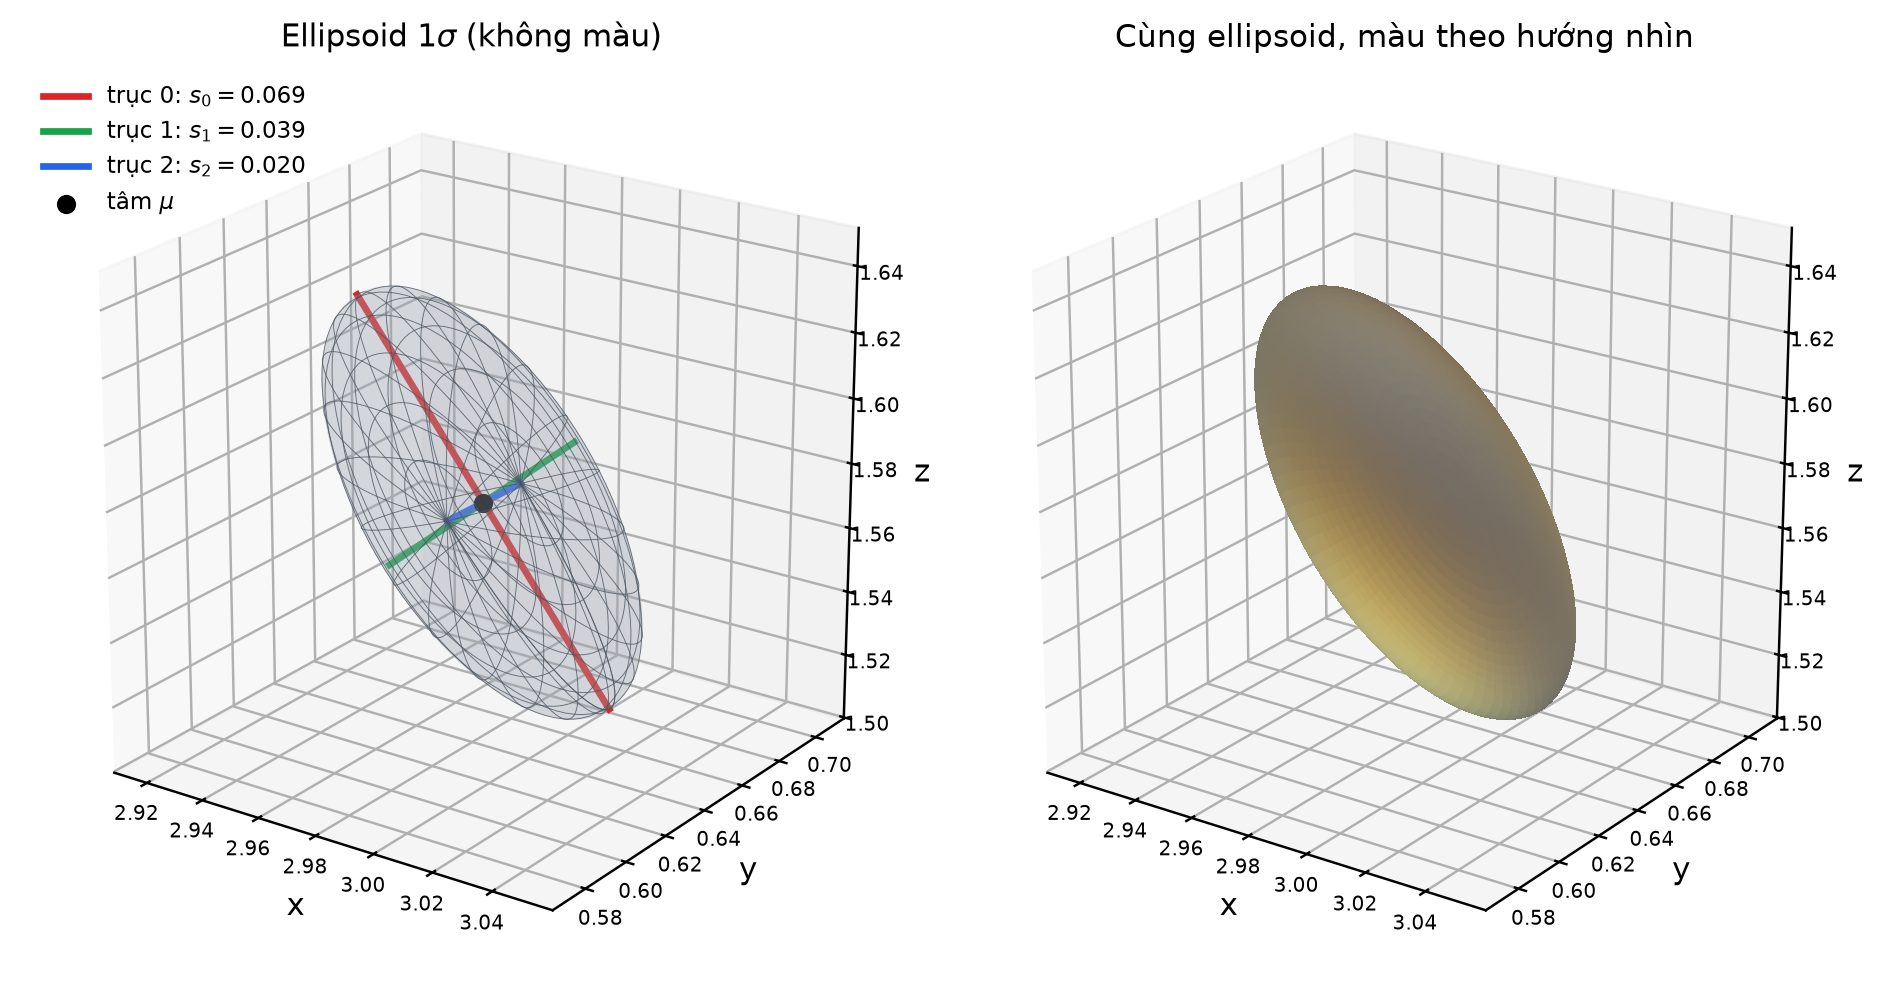
\includegraphics[width=\columnwidth]{figures/example_ellipsoid.png}
\caption{One gaussian from the file. Left: the $1\sigma$ ellipsoid with its three axes and its centre $\symbf{\mu}$. Right: the same ellipsoid with its view-dependent colour.}
\label{fig:ellipsoid}
\end{figure}


\begin{figure*}[t]
\centering
\begin{minipage}{0.495\textwidth}\centering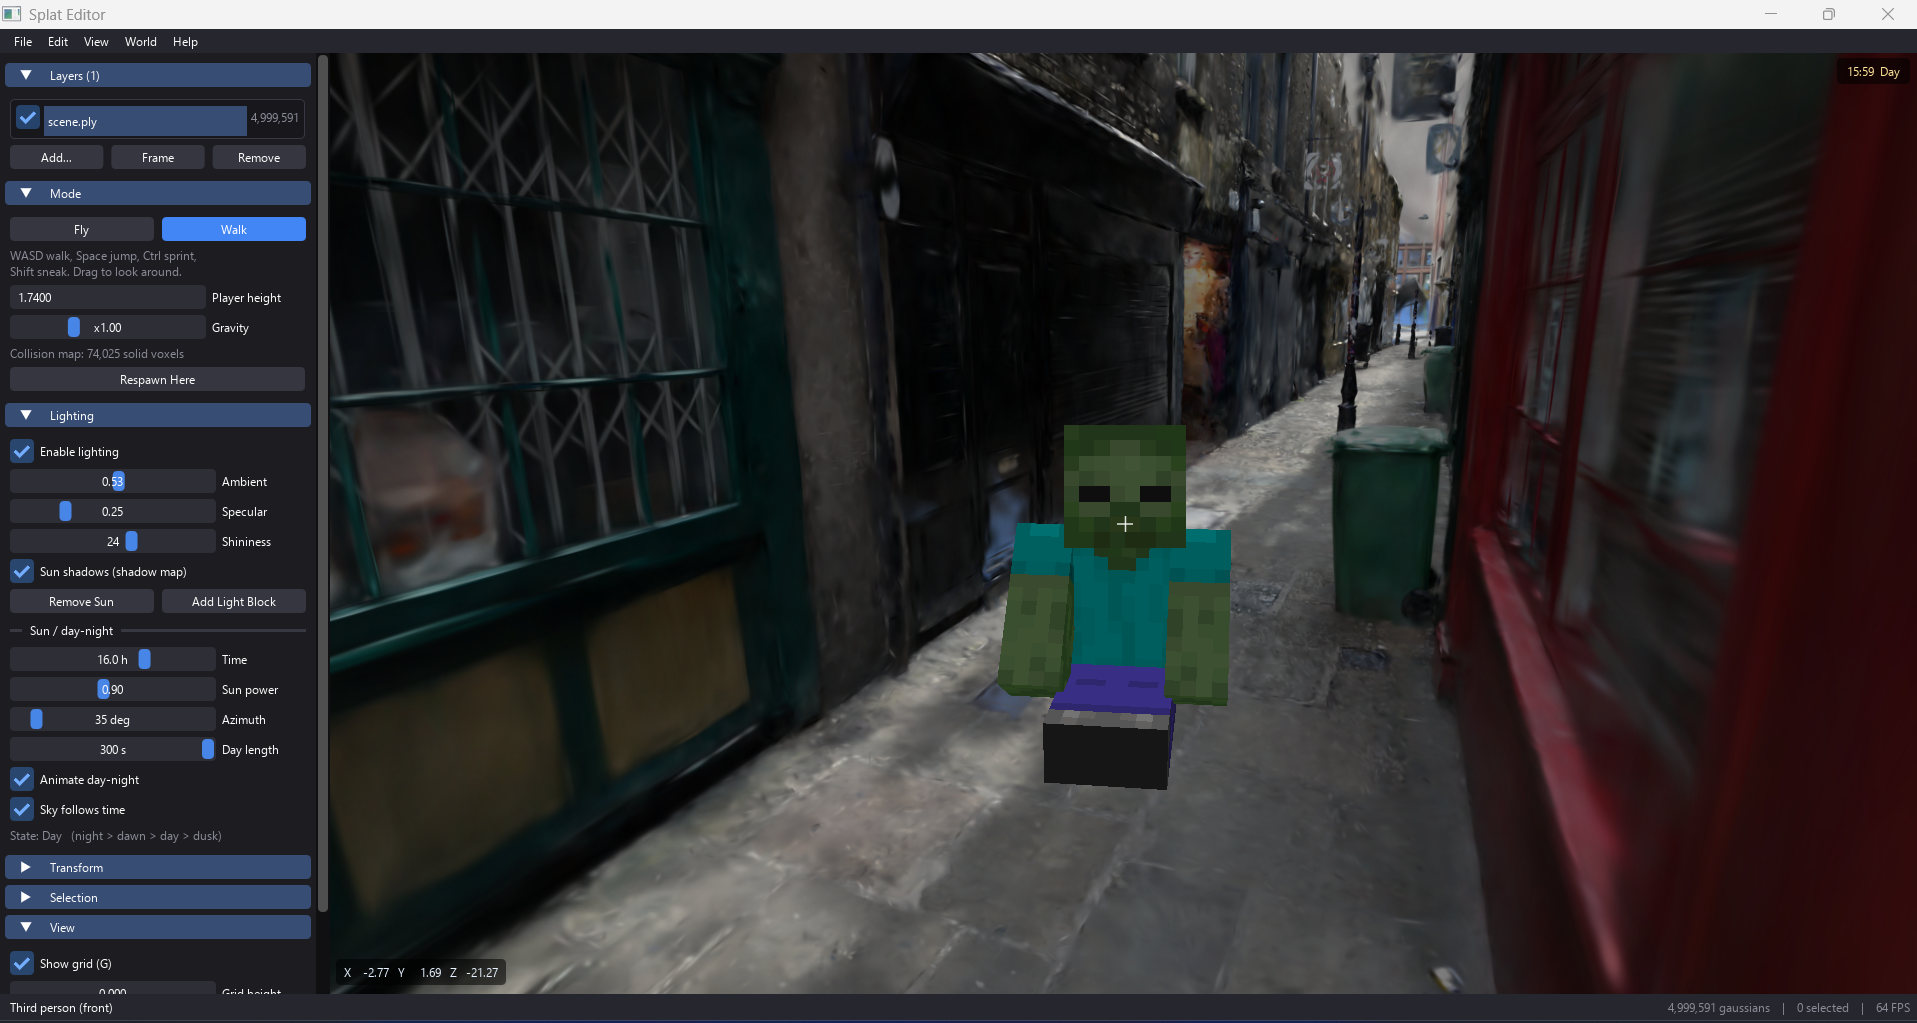
\includegraphics[width=\linewidth]{figures/t4-zombie-day.png}\\{\footnotesize (a) Day, 15:59.}\end{minipage}\hfill
\begin{minipage}{0.495\textwidth}\centering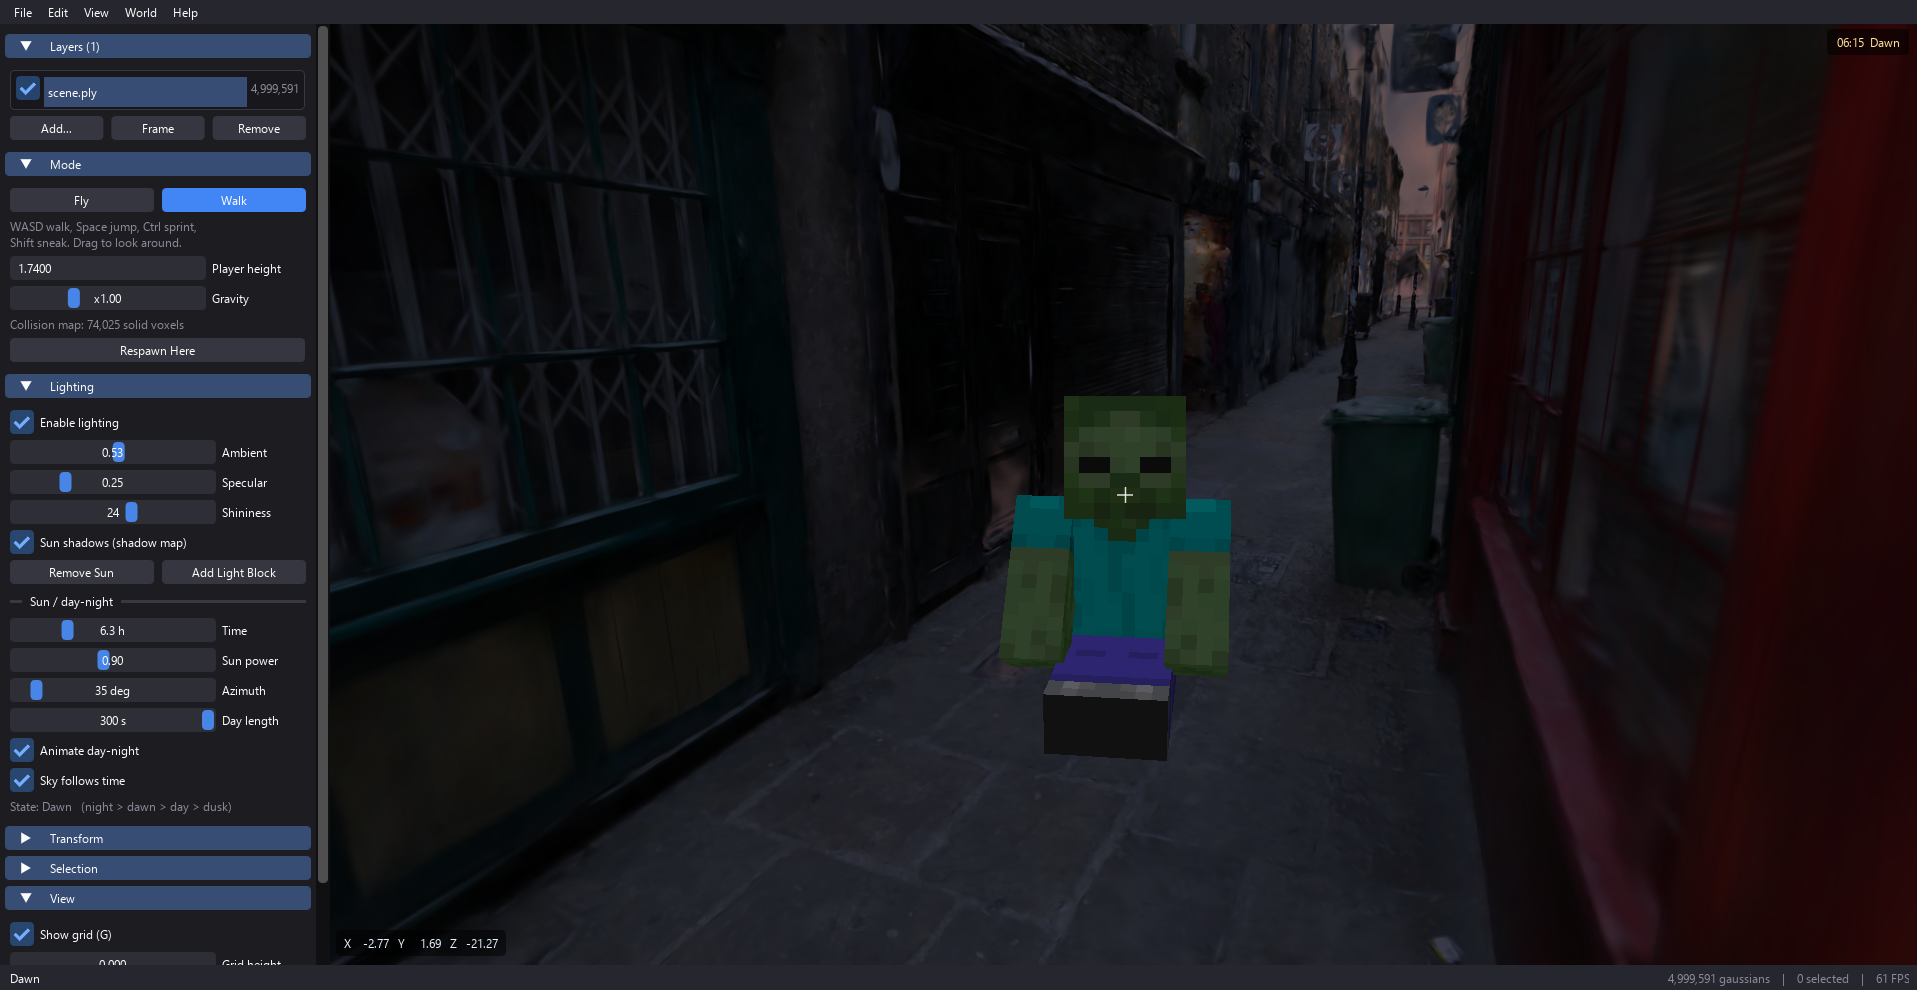
\includegraphics[width=\linewidth]{figures/t4-dawn.png}\\{\footnotesize (b) Dawn, 06:15.}\end{minipage}\\[5pt]
\begin{minipage}{0.495\textwidth}\centering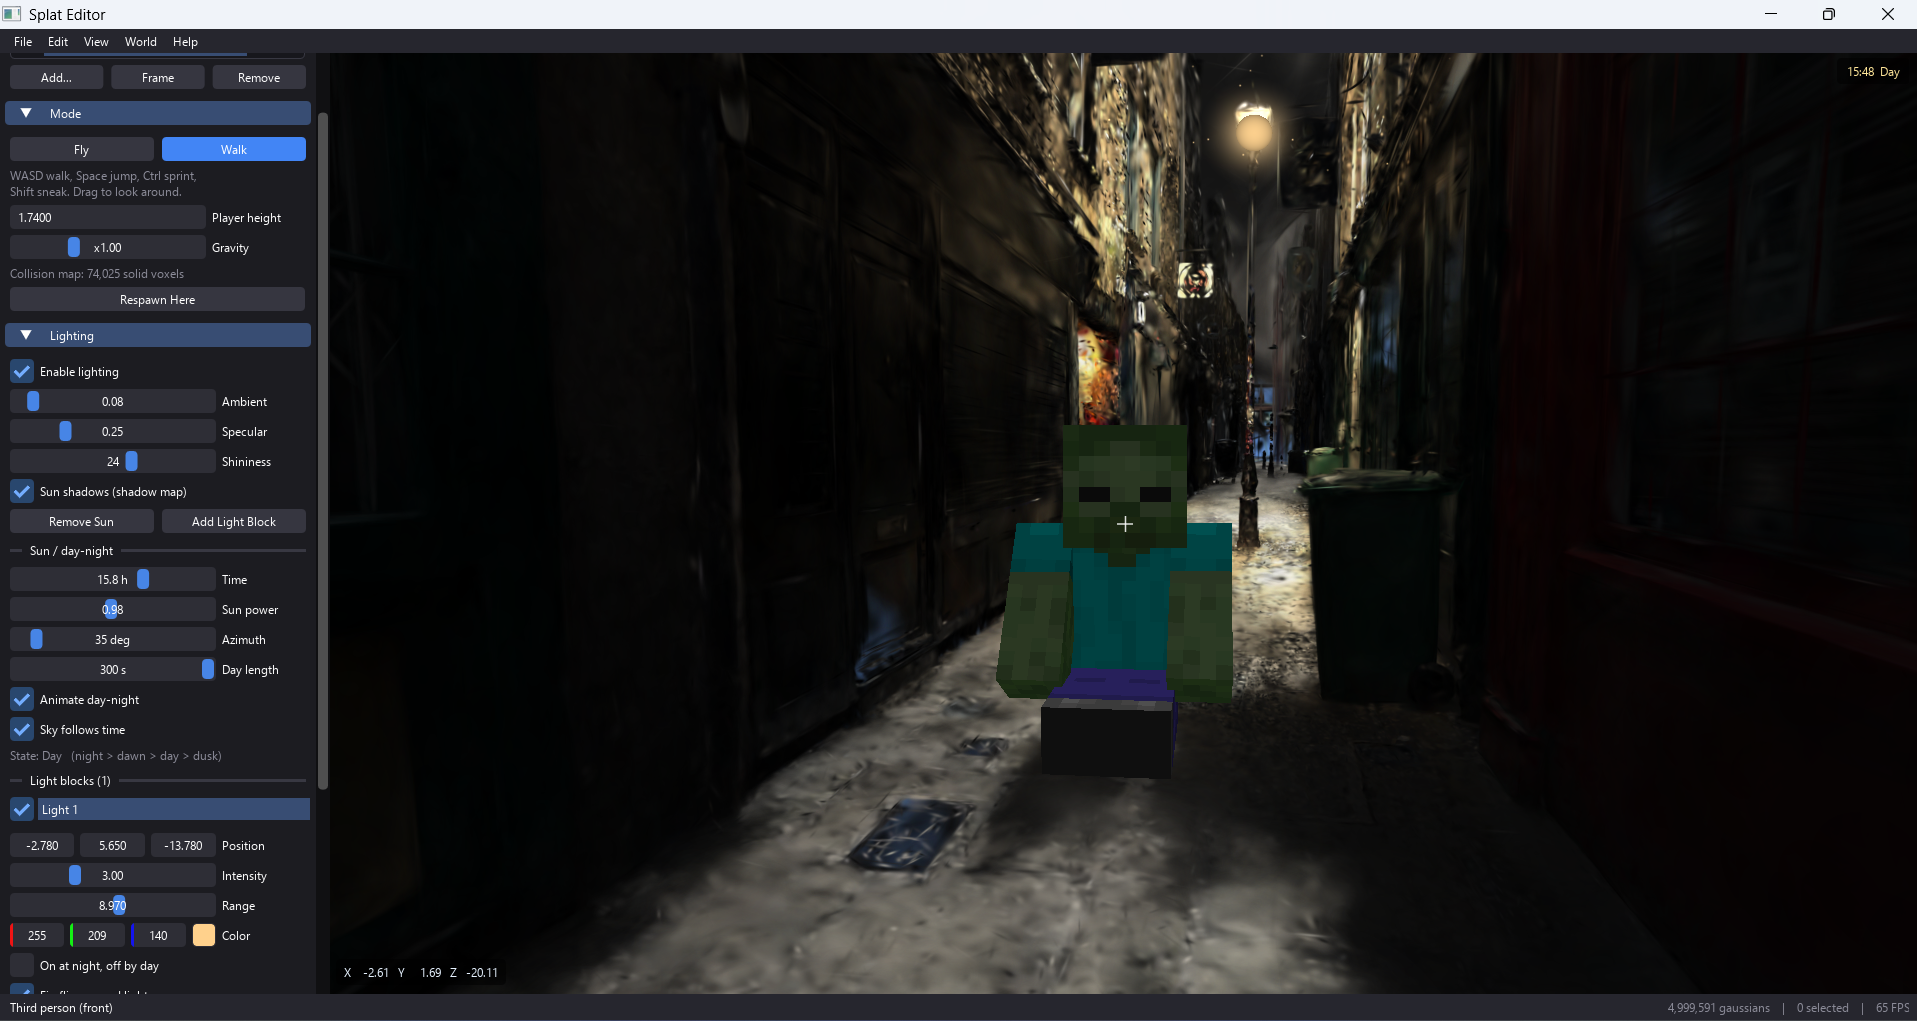
\includegraphics[width=\linewidth]{figures/t4-lamp-zombie.png}\\{\footnotesize (c) Ambient $0.08$ and a lamp.}\end{minipage}\hfill
\begin{minipage}{0.495\textwidth}\centering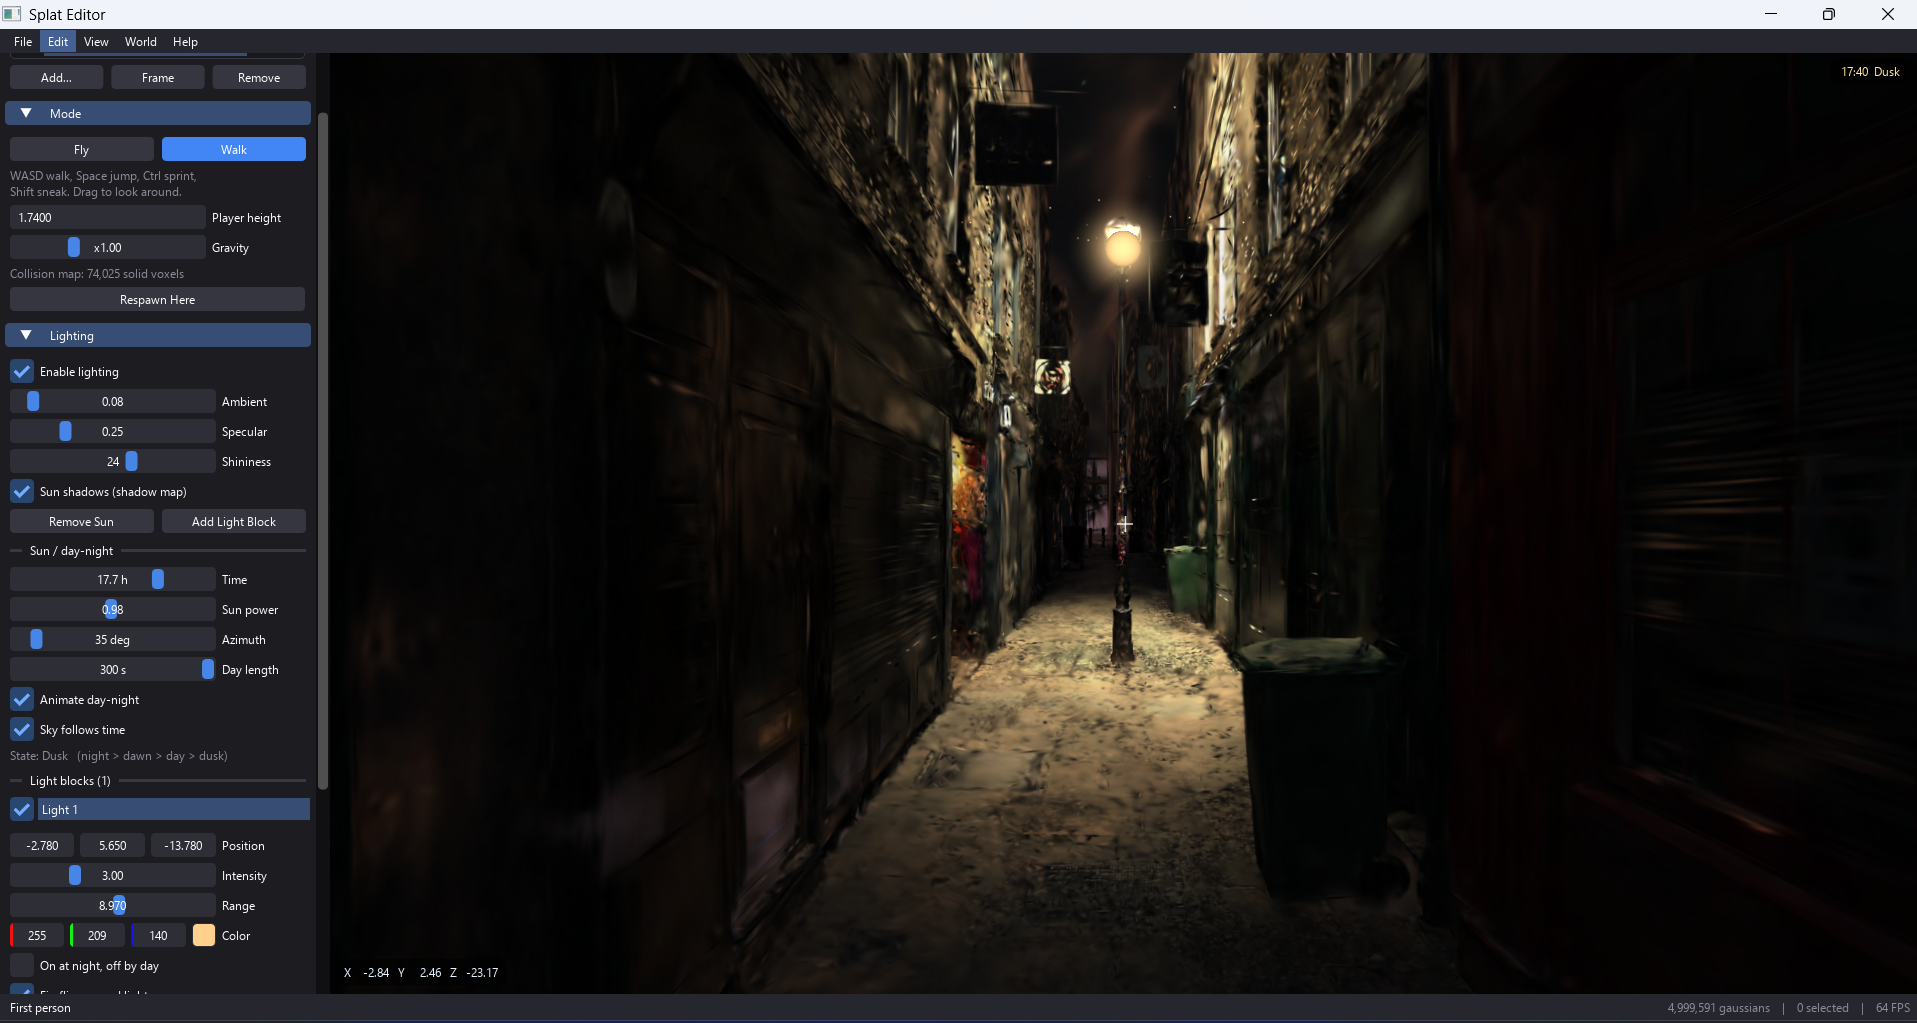
\includegraphics[width=\linewidth]{figures/t4-dusk.png}\\{\footnotesize (d) Dusk, 17:40.}\end{minipage}
\caption{A scene with the sun, one point light and the character at different times of day.}
\label{fig:t4}
\end{figure*}


%====================================================================
\section{T1: Transformations and hierarchical models}
\label{chap:t1}
%====================================================================
This chapter has two parts. Both move a whole layer.
\begin{itemize}\itemsep0pt
\item \textbf{Part 1, layer transformation.} Put a gaussian of a \code{.ply} file into the world.
\item \textbf{Part 2, rotation about a point.} Rotate a layer around a chosen centre.
\end{itemize}

\subsection{Part 1: Layer transformation}
\label{sec:layers}
Each \code{.ply} file is a layer. A layer has a translation vector $\mathbf{t}$, three Euler angles and a scale factor $s$. They form the matrix $\mathbf{M}$. This matrix takes a gaussian from file space to world space:
\begin{equation}
\mathbf{p}_w=s\mathbf{A}\mathbf{p}_f+\mathbf{t},\qquad
\Sig_w=s^{2}\mathbf{A}\,\Sig_f\,\mathbf{A}^{\top}.
\label{eq:world}
\end{equation}
Here $\mathbf{A}=\mathbf{R}_z\mathbf{R}_y\mathbf{R}_x\mathbf{F}$. $\mathbf{F}=\mathrm{diag}(-1,-1,1)$ is an optional flip for COLMAP files, whose $Y$ axis points down. The gaussian data does not change. Only $\mathbf{M}$ changes. So moving, rotating or scaling a layer is instant. On save, the program writes the transform into every gaussian. It also rotates the SH coefficients so the view-dependent colour stays correct.

\begin{codebox}
\begin{lstlisting}[language=Python,caption={\code{core/math3d.py} and \code{core/layer.py}: the layer matrix $\mathbf{M}$},label={lst:world}]
rx = np.array([[1, 0, 0], [0, cx, -sx], [0, sx, cx]])
ry = np.array([[cy, 0, sy], [0, 1, 0], [-sy, 0, cy]])
rz = np.array([[cz, -sz, 0], [sz, cz, 0], [0, 0, 1]])
return rz @ ry @ rx

rot = self.transform.rotation_matrix() @ (FLIP if flip else np.identity(3))
m = np.identity(4)
m[:3, :3] = s * rot
m[:3, 3] = t
\end{lstlisting}
\end{codebox}

\subsection{Part 2: Rotation about a point}
A layer can rotate about a point $\mathbf{c}$ with a matrix $\symbf{\Delta}$:
\begin{equation}
\mathbf{R}'=\symbf{\Delta}\mathbf{R},\qquad \mathbf{t}'=\symbf{\Delta}(\mathbf{t}-\mathbf{c})+\mathbf{c}.
\end{equation}

\begin{codebox}
\begin{lstlisting}[language=Python,caption={\code{core/transform.py}, \code{Transform.rotate\_about}},label={lst:pivot}]
def rotate_about(self, delta, pivot):
    pivot = np.asarray(pivot, float)
    self.rotation = matrix_to_euler(delta @ self.rotation_matrix())
    self.position = list(delta @ (self.translation() - pivot) + pivot)
\end{lstlisting}
\end{codebox}

%====================================================================
\section{T2: Camera and projection}
\label{chap:t2}
%====================================================================
A gaussian goes through four steps to become pixels on the screen \cite{zwicker2002ewa}. Each step is one box in Fig.~\ref{fig:ewa}, read from left to right.
\begin{itemize}\itemsep0pt
\item \textbf{Part 1, viewing transformation.} Move the gaussian from object space to camera space.
\item \textbf{Part 2, projective mapping.} Turn the 3D ellipsoid into a 2D ellipse.
\item \textbf{Part 3, shading and integration.} Compute the opacity of each pixel and blend the gaussians together.
\item \textbf{Part 4, viewport transformation.} Place the result in the viewport of the window.
\item \textbf{Part 5, three cameras.} The camera gives the input of part 1.
\end{itemize}
The five parts below follow this order.
\begin{figure}[H]
\centering
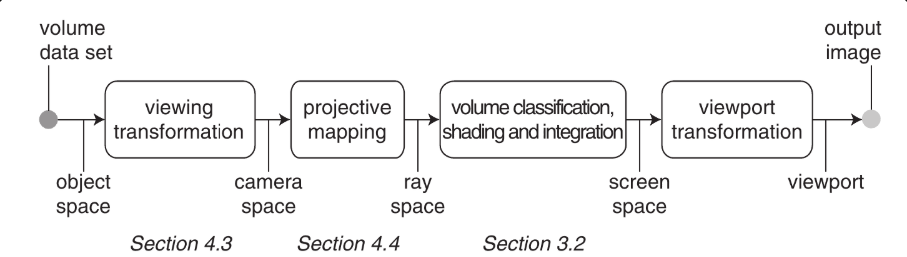
\includegraphics[width=\columnwidth]{figures/1 (3).png}
\caption{The splatting pipeline of EWA \cite{zwicker2002ewa}. The viewing transformation is $\mathbf{W}$ and the projective mapping is approximated by $\mathbf{J}$.}
\label{fig:ewa}
\end{figure}

\subsection{Part 1: Viewing transformation}
\label{sec:cam}
This step changes the coordinate system. After it, the camera is at the origin and looks along the $-z$ axis. The \code{look\_at} function builds three camera axes from the eye position $\mathbf{e}$ and the target: right $\mathbf{r}$, up $\mathbf{u}$ and forward $\mathbf{f}$. The view matrix is
\begin{equation}
\mathbf{V}=\begin{pmatrix}
\setlength{\fboxsep}{2pt}\fcolorbox{red}{white}{$\begin{matrix}
r_x&r_y&r_z\\u_x&u_y&u_z\\-f_x&-f_y&-f_z\end{matrix}$}
&\begin{matrix}-\mathbf{r}\!\cdot\!\mathbf{e}\\-\mathbf{u}\!\cdot\!\mathbf{e}\\ \mathbf{f}\!\cdot\!\mathbf{e}\end{matrix}\\[3mm]
\begin{matrix}0&0&0\end{matrix}&1\end{pmatrix}.
\label{eq:view}
\end{equation}
The centre of the gaussian is multiplied by $\mathbf{V}$. The result is the centre in camera space $(v_x,v_y,v_z)$. The shape of the gaussian is only rotated. The matrix $\mathbf{W}$ is the rotation part of $\mathbf{V}$. It is the top-left $3\times3$ block, in the red box of \eqref{eq:view}. Its rows are the three camera axes:
\begin{equation}
\mathbf{W}=\begin{pmatrix}
r_x&r_y&r_z\\u_x&u_y&u_z\\-f_x&-f_y&-f_z\end{pmatrix}.
\label{eq:W}
\end{equation}
The ellipsoid \eqref{eq:cov3d} in camera space is $\mathbf{W}\,\Sig\,\mathbf{W}^{\top}$.

\begin{codebox}
\begin{lstlisting}[language=Python,caption={\code{core/math3d.py}, \code{look\_at}: view matrix $\mathbf{V}$},label={lst:lookat}]
def look_at(eye, target, up):
    forward = target - eye
    forward /= np.linalg.norm(forward)
    right = np.cross(forward, up)
    right /= np.linalg.norm(right)
    true_up = np.cross(right, forward)
    m = np.identity(4, np.float32)
    m[0, :3] = right
    m[1, :3] = true_up
    m[2, :3] = -forward
    m[:3, 3] = -m[:3, :3] @ eye
    return m
\end{lstlisting}
\end{codebox}

\subsection{Part 2: Projective mapping}
\label{sec:ewa}
This step takes camera space to the image plane.

\textbf{Projecting a point.} The perspective matrix uses the vertical field of view $\varphi$ ($k=1/\tan(\varphi/2)$), the aspect ratio $a$, the near plane $n$ and the far plane $f$:
\begin{equation}
\mathbf{P}=\begin{pmatrix}
\frac{k}{a}&0&0&0\\0&k&0&0\\
0&0&\frac{f+n}{n-f}&\frac{2fn}{n-f}\\0&0&-1&0\end{pmatrix}.
\label{eq:proj}
\end{equation}
The point is multiplied by $\mathbf{P}$ and divided by $c_w$. The result is the normalised coordinates $(n_x,n_y)$ in the range $[-1,1]$. The division by $c_w$ makes far objects look smaller. The centre of the gaussian is projected this way.

\begin{codebox}
\begin{lstlisting}[language=Python,caption={\code{core/math3d.py}, \code{perspective}: projection matrix $\mathbf{P}$},label={lst:persp}]
def perspective(fov_y_deg, aspect, near, far):
    zoom = 1.0 / math.tan(math.radians(fov_y_deg) / 2)
    m = np.zeros((4, 4), np.float32)
    m[0, 0] = zoom / aspect
    m[1, 1] = zoom
    m[2, 2] = (far + near) / (near - far)
    m[2, 3] = 2 * far * near / (near - far)
    m[3, 2] = -1
    return m
\end{lstlisting}
\end{codebox}

\textbf{Projecting a gaussian.} A gaussian is not a point. Its ellipsoid must become an ellipse on screen. The division by $c_w$ is not linear, so we cannot multiply $\mathbf{P}$ with the ellipsoid. EWA replaces the projection by its derivative (the Jacobian) at the centre of the gaussian:
\begin{equation}
\mathbf{J}=\begin{pmatrix}
\frac{f_{px}}{-v_z}&0&\frac{f_{px}\,v_x}{v_z^{2}}\\[1mm]
0&\frac{f_{px}}{-v_z}&\frac{f_{px}\,v_y}{v_z^{2}}\\[1mm]
0&0&0
\end{pmatrix}.
\label{eq:jac}
\end{equation}
Here $f_{px}=kH/2$ is the focal length in pixels, with $k$ from \eqref{eq:proj} and $H$ the viewport height. Joining step 1 and step 2, the 2D covariance is
\begin{equation}
\Sig'=\mathbf{J}\,\mathbf{W}\,\Sig\,\mathbf{W}^{\top}\mathbf{J}^{\top}.
\label{eq:ewa}
\end{equation}
Here $\Sig$ is the 3D covariance \eqref{eq:cov3d}. $\mathbf{W}$ is the rotation part of the view matrix from step 1. $\mathbf{J}$ is the Jacobian \eqref{eq:jac}. Let the top-left $2\times2$ block of $\Sig'$ be $\begin{pmatrix}a&b\\b&c\end{pmatrix}$. Its eigenvalues are
\begin{equation}
\lambda_{1,2}=\frac{a+c}{2}\pm\sqrt{\Big(\frac{a-c}{2}\Big)^{2}+b^{2}}.
\label{eq:eig}
\end{equation}
The two semi-axes of the ellipse are proportional to $\sqrt{\lambda_1}$ and $\sqrt{\lambda_2}$. The shader draws each gaussian as a quad covering at most 3 standard deviations. It drops gaussians whose centre is behind the camera or more than $1.3$ times outside the screen.

\begin{codebox}
\begin{lstlisting}[language=GLSL,caption={\code{render/shaders/splat\_prep.vert}: Jacobian $\mathbf{J}$ and $\Sigma'=\mathbf{J}\mathbf{W}\Sigma\mathbf{W}^{\top}\mathbf{J}^{\top}$},label={lst:ewa}]
float vx = viewPos.x, vy = viewPos.y, vz = viewPos.z;
mat3 J = mat3(uFocal / -vz, 0.0, 0.0,
              0.0, uFocal / -vz, 0.0,
              uFocal * vx / (vz * vz), uFocal * vy / (vz * vz), 0.0);
mat3 T = J * mat3(uModelView) * linear;
mat3 cov = T * sigma * transpose(T);
float a = cov[0][0] + 0.3;
float b = cov[0][1];
float c = cov[1][1] + 0.3;
\end{lstlisting}
\end{codebox}

\begin{codebox}
\begin{lstlisting}[language=GLSL,caption={\code{render/shaders/splat\_prep.vert}: eigenvalues and the two ellipse axes},label={lst:eig}]
float mid = 0.5 * (a + c);
float radius = length(vec2(0.5 * (a - c), b));
float lambda1 = mid + radius;
float lambda2 = max(mid - radius, 0.1);
vec2 axis1 = (abs(b) < 1e-6) ? (a >= c ? vec2(1.0, 0.0) : vec2(0.0, 1.0))
                             : normalize(vec2(b, lambda1 - a));
vec2 axis2 = vec2(-axis1.y, axis1.x);
vec2 major = min(extent * sqrt(lambda1), 1024.0) * axis1 * toNdc;
vec2 minor = min(extent * sqrt(lambda2), 1024.0) * axis2 * toNdc;
\end{lstlisting}
\end{codebox}

\subsection{Part 3: Shading and alpha blending}
\label{sec:blend}
This step gives each pixel a colour. The fragment shader visits each pixel $\mathbf{x}$ of the quad. It evaluates the 2D Gaussian function at $\mathbf{x}$. The centre $\symbf{\mu}'$ is the projected gaussian centre. The covariance $\Sig'$ comes from \eqref{eq:ewa}:
\begin{equation}
G(\mathbf{x})=\exp\!\Big(-\tfrac12(\mathbf{x}-\symbf{\mu}')^{\top}\,\Sig'^{-1}\,(\mathbf{x}-\symbf{\mu}')\Big).
\label{eq:gauss}
\end{equation}
The exponent is $-r^2/2$. Here $r$ is the distance to the ellipse centre, in standard deviations. The opacity of gaussian $i$ at the pixel is $a_i=\alpha_i\,G_i(\mathbf{x})$.

\begin{codebox}
\begin{lstlisting}[language=GLSL,caption={\code{render/shaders/splat.frag}: $a=\alpha\,e^{-r^2/2}$},label={lst:frag}]
float r2 = dot(vCorner, vCorner);
if (r2 > 9.0) discard;
float alpha = vColor.a * exp(-0.5 * r2);
if (alpha < 1.0 / 255.0) discard;
fragColor = vec4(vColor.rgb * alpha, alpha);
\end{lstlisting}
\end{codebox}

The gaussians are drawn from far to near and blended. The pixel colour is
\begin{equation}
\mathbf{C}=\sum_{i}\mathbf{c}_i\,a_i\,T_i,\qquad
T_i=\prod_{j<i}(1-a_j),
\label{eq:over}
\end{equation}
Here the gaussians are numbered from near to far. $T_i$ is the transmittance. It is the fraction of light left after passing through the gaussians nearer than $i$.

The program draws from far to near. It gets the same result with the blend $\mathbf{C}\leftarrow\mathbf{c}\,a+(1-a)\,\mathbf{C}$ for each splat. Here $\mathbf{C}$ is the accumulated colour.

The result depends on the order. So we must sort by depth. The program converts depth to 16 bits. It sorts with NumPy in a background thread. Until the sort is done, it draws with the order of the previous sort. The depth test is turned off. The reason is that a transparent gaussian must not hide the gaussians behind it.

\begin{codebox}
\begin{lstlisting}[language=Python,caption={\code{render/splat\_renderer.py}: the blend $\mathbf{C}\leftarrow\mathbf{c}a+(1-a)\mathbf{C}$},label={lst:blend}]
GL.glDisable(GL.GL_DEPTH_TEST)
GL.glEnable(GL.GL_BLEND)
GL.glBlendFunc(GL.GL_ONE, GL.GL_ONE_MINUS_SRC_ALPHA)
GL.glDrawArraysInstanced(GL.GL_TRIANGLE_STRIP, 0, 4, self.draw_count)
\end{lstlisting}
\end{codebox}

\begin{codebox}
\begin{lstlisting}[language=Python,caption={\code{render/sorter.py}, \code{DepthSorter.sort}: far-to-near order},label={lst:sort}]
depth[start:start + count] = positions[start:start + count] @ row[:3] + row[3]
visible = np.flatnonzero(depth < 0)
far_z, near_z = float(depth.min()), float(depth.max())
scale = 65535.0 / (near_z - far_z) if near_z > far_z else 0.0
depth_key = ((depth - far_z) * scale).astype(np.uint16)
return visible[np.argsort(depth_key, kind='stable')].astype(np.uint32)
\end{lstlisting}
\end{codebox}

\subsection{Part 4: Viewport transformation}
\label{sec:viewport}
The last step converts the normalised coordinates $(n_x,n_y)$ of step 2 to pixels. The viewport has size $W\times H$ and corner $(x_0,y_0)$:
\begin{equation}
x_{px}=x_0+\tfrac{n_x+1}{2}W,\qquad y_{px}=y_0+\tfrac{1-n_y}{2}H.
\label{eq:pixel}
\end{equation}
OpenGL does this step itself when drawing. The program also uses this formula to know which pixel a gaussian is on, for example in brush selection (Section~\ref{chap:t6}).

\begin{codebox}
\begin{lstlisting}[language=Python,caption={\code{editor/brush.py}, \code{BrushTool.\_to\_screen}: clip space to pixels},label={lst:pixel}]
def _to_screen(clip, viewport):
    left, top, width, height = viewport
    x = left + (clip[..., 0] / clip[..., 3] + 1) * 0.5 * width
    y = top + (1 - clip[..., 1] / clip[..., 3]) * 0.5 * height
    return x, y
\end{lstlisting}
\end{codebox}

\subsection{Part 5: Three cameras}
\textbf{Orbit camera.} The camera always looks at a point $\mathbf{t}$. Its position uses a yaw angle $\theta$, a pitch angle $\phi$ and a distance $d$:
\begin{equation}
\mathbf{e}=\mathbf{t}+d\,(\cos\phi\sin\theta,\ \sin\phi,\ \cos\phi\cos\theta).
\label{eq:eye}
\end{equation}
The pitch is limited to about $\pm89^{\circ}$ so the camera does not flip.

\begin{codebox}
\begin{lstlisting}[language=Python,caption={\code{render/camera.py}, \code{OrbitCamera.position}},label={lst:eye}]
PITCH_LIMIT = 1.55
cp = math.cos(self.pitch)
offset = np.array([cp * math.sin(self.yaw), math.sin(self.pitch),
                   cp * math.cos(self.yaw)])
return self.target + self.distance * offset
\end{lstlisting}
\end{codebox}

\textbf{Fly camera.} The velocity does not change at once. It moves gradually to the wanted velocity $\mathbf{v}^{*}$, so the camera has inertia:
\begin{equation}
\mathbf{v}\leftarrow\mathbf{v}+(\mathbf{v}^{*}-\mathbf{v})\min(10\Delta t,1),\qquad
\mathbf{e}\leftarrow\mathbf{e}+\mathbf{v}\,\Delta t.
\label{eq:fly}
\end{equation}

\begin{codebox}
\begin{lstlisting}[language=Python,caption={\code{render/camera.py}, \code{OrbitCamera.fly}},label={lst:fly}]
wanted = direction * self.fly_speed * (self.SPRINT_FACTOR if sprint else 1.0)
self.velocity += (wanted - self.velocity) * min(self.FLY_ACCEL * dt, 1.0)
self.target += self.velocity * dt
\end{lstlisting}
\end{codebox}



%====================================================================
\section{T3: Texture mapping}
\label{chap:t3}
%====================================================================
The program uses a texture to paint the box model of the character with a skin image. The character has 6 boxes (head, body, two arms and two legs). The skin is a $64\times64$ image (Fig.~\ref{fig:skin}) that holds the unfolded faces of all 6 boxes in the Minecraft cross layout. Each face of a box only has to take its own cell of the image. There are three steps (Fig.~\ref{fig:skinflow}).

\begin{figure}[H]
\centering
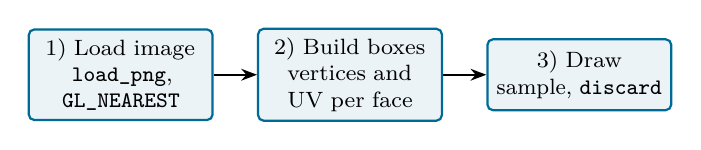
\begin{tikzpicture}[node distance=5.5mm]
\node[pbox] (a) {1) Load image \\ \code{load\_png}, \code{GL\_NEAREST}};
\node[pbox,right=of a] (b) {2) Build boxes \\ vertices and UV per face};
\node[pbox,right=of b] (c) {3) Draw \\ sample, \code{discard}};
\draw[parr] (a)--(b); \draw[parr] (b)--(c);
\end{tikzpicture}
\caption{Three steps to draw the skin.}
\label{fig:skinflow}
\end{figure}

\textbf{1) Build the box.} A box has centre $\mathbf{c}$, size $(w,h,d)$ and inflation $\delta$. Each corner of a face is
$\mathbf{p}=\mathbf{c}+\big(s_x(\tfrac w2+\delta),\,s_y(\tfrac h2+\delta),\,s_z(\tfrac d2+\delta)\big)$, $s_x,s_y,s_z\in\{\pm1\}$.
The box is built twice: a base layer ($\delta=0$) and an overlay layer ($\delta=0.25$ for body and limbs, $0.5$ for the hat). The overlay is slightly larger, so it does not stick to the base layer.

\begin{codebox}
\begin{lstlisting}[language=Python,caption={\code{render/avatar\_renderer.py}, \code{\_box}: corner $\mathbf{p}$ of a face},label={lst:boxcorner}]
(cx, cy, cz), (w, h, d) = centre, size
hx, hy, hz = w / 2 + inflate, h / 2 + inflate, d / 2 + inflate
...
for (sx, sy, sz), (u, v) in zip(_FACES[face], uvs):
    vertices.append((cx + sx * hx, cy + sy * hy, cz + sz * hz, ...))
\end{lstlisting}
\end{codebox}

\textbf{2) Pick the cell in the image.} A box has origin $(o_x,o_y)$ in the skin. Fig.~\ref{fig:skincross} shows where the six faces are. For example, the head has origin $(0,0)$ and $w=h=d=8$, so its front face (the face of the character) is in the cell $(8,8,8,8)$. The four corners of a cell $(r_x,r_y,r_w,r_h)$ get the UV
\begin{equation}
(u,v)=\Big(\tfrac{r_x+k\,r_w}{64},\,\tfrac{r_y+l\,r_h}{64}\Big),\quad (k,l)\in\{(0,0),(1,0),(1,1),(0,1)\}.
\label{eq:skin-uv}
\end{equation}
The order of the four corners must match the order of the four vertices of the face. If they differ, the image is flipped or rotated.

\begin{codebox}
\begin{lstlisting}[language=Python,caption={\code{render/avatar\_renderer.py}: skin cell and UV of a face},label={lst:skinuv}]
def _uv_region(face, ox, oy, w, h, d):
    return ((ox + d, oy + d, w, h), (ox + 2 * d + w, oy + d, w, h),
            (ox, oy + d, d, h), (ox + d + w, oy + d, d, h),
            (ox + d, oy, w, d), (ox + d + w, oy, w, d))[face]

rx, ry, rw, rh = _uv_region(face, ox, oy, w, h, d)
uvs = ((rx, ry), (rx + rw, ry), (rx + rw, ry + rh), (rx, ry + rh))
...  u / SKIN_SIZE, v / SKIN_SIZE
\end{lstlisting}
\end{codebox}

\begin{figure}[H]
\centering
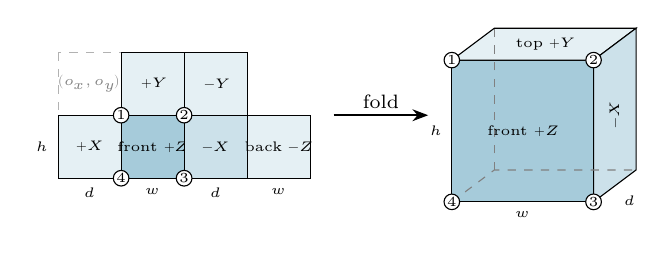
\begin{tikzpicture}[font=\tiny]
% hình chữ thập trên ảnh skin (gốc (o_x,o_y) ở góc trên trái)
\begin{scope}[x=0.4cm,y=-0.4cm]
\draw[dashed,gray!60] (0,0) rectangle (2,2);
\node[gray] at (1,1) {$(o_x,o_y)$};
\draw[fill=linkblue!10] (2,0) rectangle (4,2) node[midway]{$+Y$};
\draw[fill=linkblue!10] (4,0) rectangle (6,2) node[midway]{$-Y$};
\draw[fill=linkblue!10] (0,2) rectangle (2,4) node[midway]{$+X$};
\draw[fill=linkblue!35] (2,2) rectangle (4,4) node[midway]{front $+Z$};
\draw[fill=linkblue!20] (4,2) rectangle (6,4) node[midway]{$-X$};
\draw[fill=linkblue!10] (6,2) rectangle (8,4) node[midway]{back $-Z$};
\foreach \p/\n in {{2,2}/1,{4,2}/2,{4,4}/3,{2,4}/4}
  \node[circle,fill=white,draw,inner sep=0.3pt] at (\p) {\n};
\node[below] at (1,4) {$d$}; \node[below] at (3,4) {$w$};
\node[below] at (5,4) {$d$}; \node[below] at (7,4) {$w$};
\node[left] at (0,3) {$h$};
\end{scope}
\draw[parr] (3.5,-0.8) -- node[plab,above=1pt]{fold} (4.7,-0.8);
% hộp 3D tương ứng (phép chiếu xiên)
\begin{scope}[shift={(5.0,-1.9)},x=0.9cm,y=0.9cm]
\draw[fill=linkblue!35] (0,0) rectangle (2,2);
\draw[fill=linkblue!10] (0,2) -- (2,2) -- (2.6,2.45) -- (0.6,2.45) -- cycle;
\draw[fill=linkblue!20] (2,0) -- (2.6,0.45) -- (2.6,2.45) -- (2,2) -- cycle;
\draw[dashed,gray] (0,0) -- (0.6,0.45) -- (2.6,0.45); \draw[dashed,gray] (0.6,0.45) -- (0.6,2.45);
\node at (1,1) {front $+Z$};
\node at (1.3,2.22) {top $+Y$};
\node[rotate=90] at (2.3,1.22) {$-X$};
\foreach \p/\n in {{0,2}/1,{2,2}/2,{2,0}/3,{0,0}/4}
  \node[circle,fill=white,draw,inner sep=0.3pt] at (\p) {\n};
\node[below] at (1,0) {$w$}; \node[left] at (0,1) {$h$};
\node[below right] at (2.3,0.22) {$d$};
\end{scope}
\end{tikzpicture}
\caption{A 3D box and its cross layout. The $+Z$ face ($w\times h$) has the cell $(o_x{+}d,\,o_y{+}d,\,w,\,h)$ and the $+Y$ face has the cell $(o_x{+}d,\,o_y,\,w,\,d)$. The corners 1, 2, 3, 4 of each face get $(k,l)=(0,0),(1,0),(1,1),(0,1)$ in \eqref{eq:skin-uv}.}
\label{fig:skincross}
\end{figure}

\textbf{3) Draw.} The skin is loaded by my own \code{load\_png} function and filtered with \code{GL\_NEAREST}, so the pixels stay sharp ($\lfloor 64u\rfloor,\lfloor 64v\rfloor$). The fragment shader discards pixels with $\alpha<0.5$, so the transparent parts of the overlay show the base layer. The final colour is the texel times $0.62+0.38\max(\mathbf{n}\!\cdot\!\mathbf{l},0)$. Each box is drawn with its own model matrix, so arms and legs rotate independently about their joints.

\begin{figure}[H]
\centering
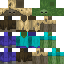
\includegraphics[width=0.45\columnwidth]{figures/skinzom.png}
\caption{The $64\times64$ skin of the character. Each box (head, body, arms, legs) has one cross for the base layer and one for the overlay (hat, jacket, sleeves).}
\label{fig:skin}
\end{figure}

%====================================================================
\section{T4: Lighting and shadows}
\label{chap:t4}
%====================================================================
The final colour of a gaussian is made in four parts.
\begin{itemize}\itemsep0pt
\item \textbf{Part 1, view-dependent colour.} Read the base colour from the SH coefficients.
\item \textbf{Part 2, Phong lighting.} Add ambient, diffuse and specular light.
\item \textbf{Part 3, the sun.} Move the sun and the sky colour with the hour.
\item \textbf{Part 4, shadows.} Test each gaussian against a shadow map.
\end{itemize}

\subsection{Part 1: View-dependent colour}
\label{sec:sh}
The colour of a gaussian changes with the view direction $\mathbf{d}$. 3DGS stores this with spherical harmonics (SH) coefficients \cite{kerbl2023gaussian}:
\begin{equation}
\mathbf{c}(\mathbf{d})=\operatorname{clip}\!\Big(\mathbf{c}_0+\sum_{k=1}^{K}Y_k(\mathbf{d})\,\mathbf{h}_k,\,0,\,1\Big).
\label{eq:sh}
\end{equation}
Here $\mathbf{c}_0$ is the base colour, $\mathbf{h}_k$ are the coefficients in the file and $Y_k$ are the basis functions. The coefficients are in file space. So the shader rotates the view direction into that space: $\mathbf{d}=\operatorname{norm}\!\big(\mathbf{A}^{\top}(\mathbf{p}_w-\mathbf{e})\big)$. It does not have to rotate the coefficients every frame. Fig.~\ref{fig:sh} shows the idea for degrees 0 to 2. Each basis function is a pattern on the sphere. The weighted sum gives one colour for each view direction.

\begin{codebox}
\begin{lstlisting}[language=GLSL,caption={\code{render/shaders/splat\_prep.vert}: view-dependent SH colour},label={lst:sh}]
vec3 c = -0.4886025119029199 * y * shCoeff(splat, 0)
       +  0.4886025119029199 * z * shCoeff(splat, 1)
       -  0.4886025119029199 * x * shCoeff(splat, 2);
...
vec3 color = vec3(rg, ba.x);
if (uShDegree > 0)
    color += shColor(splat, normalize(transpose(linear)
                                      * (center - uCamPos)));
color = clamp(color, 0.0, 1.0);
\end{lstlisting}
\end{codebox}

\begin{figure}[H]
\centering
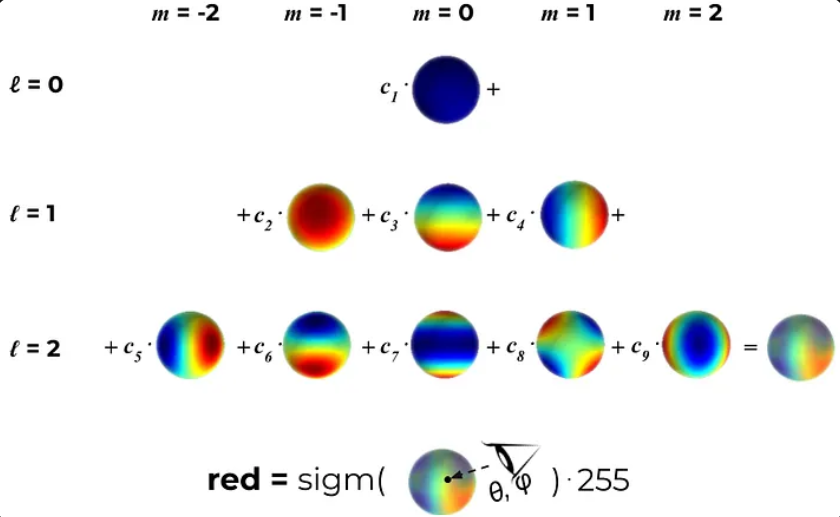
\includegraphics[width=0.8\columnwidth]{figures/1 (1).png}
\caption{Spherical harmonics up to degree 2. The nine basis functions are weighted by the coefficients $c_1..c_9$ and added. The colour is read at the view direction $(\theta,\varphi)$.}
\label{fig:sh}
\end{figure}

\subsection{Part 2: Phong lighting}
Lighting is computed once per gaussian. The normal $\mathbf{n}$ is the shortest axis of the ellipsoid, flipped towards the camera. The final colour uses the Phong model \cite{phong1975}. It has three parts (Fig.~\ref{fig:phong}). Let $\mathbf{c}$ be the colour of the gaussian.

\textbf{Ambient.} The ambient light $\mathbf{L}_a$ reaches every gaussian equally:
\begin{equation}
\mathbf{I}_a=\mathbf{c}\,\mathbf{L}_a.
\label{eq:phong-a}
\end{equation}

\textbf{Diffuse.} A surface that faces the light is brighter. For light $j$, $\mathbf{L}_j$ is its colour and $\mathbf{l}_j$ is the direction to the light:
\begin{equation}
\begin{aligned}
\mathbf{I}_d&=\mathbf{c}\sum_j \mathbf{L}_j\,w(\mathbf{n},\mathbf{l}_j)\,S_j,\\
w(\mathbf{n},\mathbf{l})&=\operatorname{clip}\!\Big(\frac{\mathbf{n}\!\cdot\!\mathbf{l}+0.35}{1.35},0,1\Big).
\end{aligned}
\label{eq:phong-d}
\end{equation}
The term $w$ is a softened $\mathbf{n}\!\cdot\!\mathbf{l}$, because the estimated normal is noisy.

\textbf{Specular.} A highlight appears where the reflected ray $\mathbf{r}_j$ is close to the direction $\mathbf{v}$ to the camera:
\begin{equation}
\mathbf{I}_s=k_s\sum_{j}\mathbf{L}_j\,(\mathbf{r}_j\!\cdot\!\mathbf{v})_{+}^{m}\,S_j.
\label{eq:phong-s}
\end{equation}
Here $k_s$ is the specular strength and $m$ is the shininess. This part does not use the colour $\mathbf{c}$. It is zero when $\mathbf{n}\!\cdot\!\mathbf{l}_j\le0$.

\textbf{Sum.} The final colour is the sum of the three parts:
\begin{equation}
\mathbf{c}_{out}=\mathbf{I}_a+\mathbf{I}_d+\mathbf{I}_s.
\label{eq:phong-wrap}
\end{equation}
$S_j$ is the shadow factor of the sun, or the distance falloff of a point light. The scene has one sun and up to 8 point lights. Point lights cast no shadows.

\begin{codebox}
\begin{lstlisting}[language=GLSL,caption={\code{render/shaders/splat\_prep.vert}, \code{shade}: Phong lighting},label={lst:phong}]
vec3 diffuse = uAmbient;
vec3 spec = vec3(0.0);
float ndl = dot(n, uSunDir);
float shadow = shadowFactor(worldPos, n);
diffuse += uSunColor * shadow
         * clamp((ndl + 0.35) / 1.35, 0.0, 1.0);
if (ndl > 0.0)
    spec += uSunColor * shadow * pow(max(dot(
        reflect(-uSunDir, n), v), 0.0), uShininess);
...
return albedo * diffuse + spec * uSpecular;
\end{lstlisting}
\end{codebox}

\begin{figure}[H]
\centering
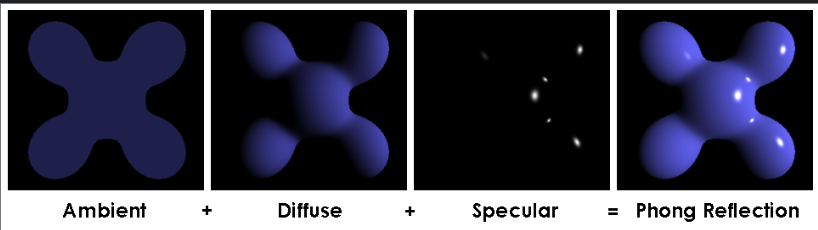
\includegraphics[width=\columnwidth]{figures/1 (2).png}
\caption{The Phong model \cite{phong1975}: ambient, diffuse and specular parts, and their sum.}
\label{fig:phong}
\end{figure}


\subsection{Part 3: The sun}
The sun direction is computed from the hour $h$ of the day. The sun rises at 6, is highest at 12 and sets at 18. The sky colour and the ambient light change gradually between day and night. They are slightly orange at dusk (Fig.~\ref{fig:t4}).

\subsection{Part 4: Shadows}
The program draws the centres of the solid gaussians as points into a $2048^2$ depth map seen from the sun \cite{williams1978}. Each gaussian is projected into this map to compare depths. If something is closer to the sun, the gaussian is in shadow. The program averages $3\times3$ samples to soften the shadow edge (PCF \cite{reeves1987}):
\begin{equation}
S=\frac19\sum_{i,j=-1}^{1}\big[\,z_s-b\le D_s(u_s+i\tau,\,v_s+j\tau)\,\big].
\label{eq:pcf}
\end{equation}
Here $(u_s,v_s,z_s)$ are the coordinates of the gaussian in the map, $D_s$ is the stored depth, $\tau$ is the texel step and $b$ is the bias. The bias stops a gaussian from shadowing itself.

\begin{codebox}
\begin{lstlisting}[language=GLSL,caption={\code{render/shaders/splat\_prep.vert}, \code{shadowFactor}: $3\times3$ PCF},label={lst:pcf}]
vec4 lp = uLightVP * vec4(worldPos + n * uShadowTexel * 2.0, 1.0);
vec3 s = lp.xyz / lp.w * 0.5 + 0.5;
float lit = 0.0;
for (int i = -1; i <= 1; i++)
    for (int j = -1; j <= 1; j++) {
        vec2 uv = s.xy + vec2(i, j) * uShadowInv;
        float d = textureLod(uShadowMap, uv, 0.0).r;
        lit += (s.z - uShadowBias <= d) ? 1.0 : 0.0;
    }
return lit / 9.0;
\end{lstlisting}
\end{codebox}

\begin{codebox}
\begin{lstlisting}[language=Python,caption={\code{core/lighting.py}, \code{Lighting.shadow\_setup}: view matrix from the sun},label={lst:shadowsetup}]
d = self.sun_direction()
r = self.radius * 1.1
eye = self.center + d * 2.0 * r
view = look_at(eye, self.center, up)
proj = orthographic(r, 0.01 * r, 4.0 * r)
return (proj @ view).astype(np.float32), texel, bias
\end{lstlisting}
\end{codebox}

%====================================================================
\section{T5: Animation and simulation}
\label{chap:t5}
%====================================================================
Every motion is multiplied by the frame time $\Delta t$. So the speed depends little on the machine. There are three parts, in the order of one frame.
\begin{itemize}\itemsep0pt
\item \textbf{Part 1, day--night cycle.} Advance the clock and move the sun.
\item \textbf{Part 2, voxel collision.} Turn the gaussians into solid voxels.
\item \textbf{Part 3, the player.} Walk, jump and fall on the voxels.
\end{itemize}

\subsection{Part 1: Day--night cycle}
This is a state machine with 4 states: NIGHT $\to$ DAWN $\to$ DAY $\to$ DUSK. The clock runs by itself. Lights set to ``on at night'' turn on at dusk and off at dawn. The states start at hour 5 (DAWN), 7 (DAY), 17 (DUSK) and 19 (NIGHT). One day lasts $T_{day}=36$ s, so the hour advances by $\Delta h = 24\,\Delta t/T_{day}$ each frame. The sun position follows the hour:
\begin{equation}
\begin{gathered}
\theta=\frac{h-6}{12}\pi,\qquad
\epsilon=65^{\circ}\sin\theta,\
\mathbf{s}=\big(\cos\epsilon\cos\phi,\;\sin\epsilon,\;\cos\epsilon\sin\phi\big),
\end{gathered}
\label{eq:sun}
\end{equation}
where $\phi=\phi_0+\theta-\pi/2$ and $\phi_0$ is the sun azimuth. The sun rises at 6, is highest at 12 and sets at 18. The daylight factor is $D=\operatorname{smoothstep}(-0.08,\,0.3,\,s_y)$. The ambient colour and the sky colour are mixed between a night value and a day value with $D$, and the sky gets an orange tint near the horizon.

\begin{codebox}
\begin{lstlisting}[language=Python,caption={\code{core/lighting.py}: hour, sun direction and daylight factor},label={lst:sun}]
hours_per_second = 24.0 / max(self.day_length, 1.0)
self.hour = (self.hour + dt * hours_per_second) % 24.0

angle = (self.hour - 6.0) / 12.0 * math.pi
elevation = math.sin(angle) * math.radians(MAX_SUN_ELEVATION)
azimuth = (math.radians(self.sun_azimuth)
           + (angle - math.pi / 2))
return np.array([math.cos(elevation) * math.cos(azimuth),
                 math.sin(elevation),
                 math.cos(elevation) * math.sin(azimuth)])

return _smooth(-0.08, 0.3, self.sun_direction()[1])
\end{lstlisting}
\end{codebox}

\subsection{Part 2: Collision with voxels}
A gaussian has no clear surface, so direct collision is hard. The program divides space into voxels of edge $v$. A voxel with enough gaussians is solid. Each solid voxel is stored as one 64-bit integer:
\begin{equation}
\mathbf{c} = \left\lfloor \frac{\mathbf{p}-\mathbf{o}}{v} \right\rfloor,
\qquad
\text{key} = (c_x \ll 42)\,|\,(c_z \ll 21)\,|\,c_y.
\label{eq:voxel}
\end{equation}
The keys are sorted. Because $c_y$ is in the low bits, the cells of one column sit next to each other. Finding the ground under the feet takes one \code{np.searchsorted} call.

\begin{codebox}
\begin{lstlisting}[language=Python,caption={\code{core/physics.py}, \code{CollisionWorld}: voxel keys and ground search},label={lst:voxel}]
cells = np.floor((positions - self.origin) / self.voxel).astype(np.int64)
keys = (cells[:, 0] << (2 * _BITS)) | (cells[:, 2] << _BITS) | cells[:, 1]
self.keys = np.unique(keys)

idx = np.searchsorted(self.keys, query, side='right') - 1
\end{lstlisting}
\end{codebox}

\begin{figure}[H]
\centering
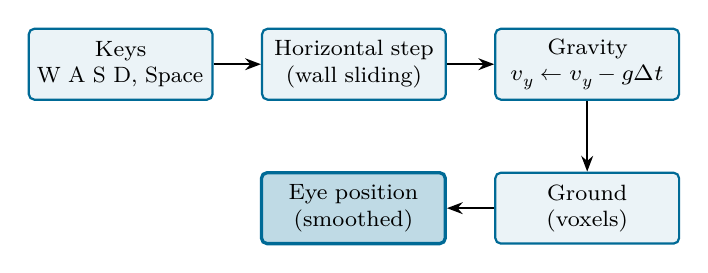
\begin{tikzpicture}[node distance=9mm and 6mm]
  \node[pbox] (key) {Keys\\W A S D, Space};
  \node[pbox,right=of key] (move) {Horizontal step\\(wall sliding)};
  \node[pbox,right=of move] (grav) {Gravity\\$v_y\leftarrow v_y-g\Delta t$};
  \node[pbox,below=of grav] (gr) {Ground\\(voxels)};
  \node[pmine,left=of gr] (eye) {Eye position\\(smoothed)};
  \draw[parr] (key) -- (move);
  \draw[parr] (move) -- (grav);
  \draw[parr] (grav) -- (gr);
  \draw[parr] (gr) -- (eye);
\end{tikzpicture}
\caption{One frame of walk mode.}
\label{fig:t5}
\end{figure}

\subsection{Part 3: The player}
Fig.~\ref{fig:t5} summarises one frame. The player is a cylinder. At a wall, the player slides along it. The player can climb a low step and can jump.

\textbf{Gravity.} When not on the ground, the program integrates with Euler steps:
\begin{equation}
v_y \leftarrow v_y - g\,\Delta t,
\qquad
y \leftarrow y + v_y\,\Delta t.
\label{eq:euler}
\end{equation}
\textbf{Scale and jump.} All sizes and speeds scale with the player height $H$. The reason is that a 3DGS scene has no fixed unit. The constants are: voxel edge $v=H/8$, player radius $0.14H$, step height $0.35H$, gravity $g=12H$, walking speed $2.5H$ per second (sprint $\times1.7$, sneak $\times0.4$). A jump reaches the height $0.75H$, so the take-off speed is
\begin{equation}
v_0=\sqrt{2\,g\,(0.75H)}.
\label{eq:jump}
\end{equation}
\textbf{Eye smoothing.} The eye height is smoothed while the player stands on the ground, so the rough gaussian surface does not shake the camera.

\begin{codebox}
\begin{lstlisting}[language=Python,caption={\code{core/physics.py}, \code{Physics.walk}: jump and gravity},label={lst:jump}]
if player.on_ground and jump:
    player.vel_y = math.sqrt(2.0 * self.gravity * self.jump_ratio * h)
    player.on_ground = False
if not player.on_ground:
    player.vel_y -= self.gravity * dt
    new_y = y + player.vel_y * dt
\end{lstlisting}
\end{codebox}

%====================================================================
\section{T6: Interaction and GUI}
\label{chap:t6}
%====================================================================
The interaction has four parts, from the input to the screen.
\begin{itemize}\itemsep0pt
\item \textbf{Part 1, event handling.} Decide who receives each mouse or keyboard event.
\item \textbf{Part 2, brush selection.} Select gaussians by painting on the screen.
\item \textbf{Part 3, soft delete and undo.} Delete the selection and restore it.
\item \textbf{Part 4, interface.} Panel, HUD and shortcuts.
\end{itemize}

\subsection{Part 1: Event handling}
Mouse and keyboard events go to ImGui first. If ImGui does not use them, they go to the camera, the selection brush and the shortcuts.

\subsection{Part 2: Brush selection}
Press \code{B} to turn on the brush. Paint on the screen to select gaussians. They turn yellow. The centre of each gaussian is projected to a pixel $\mathbf{p}$ (Section~\ref{sec:cam}). 

\textbf{Capsule test.} A stroke from $\mathbf{a}$ to $\mathbf{b}$ is a capsule of radius $r$. A gaussian is selected if
\begin{equation}
\lVert\mathbf{p}-\mathbf{a}-\tau(\mathbf{b}-\mathbf{a})\rVert\le r,\quad \tau=\operatorname{clip}\tfrac{(\mathbf{p}-\mathbf{a})\cdot(\mathbf{b}-\mathbf{a})}{\lVert\mathbf{b}-\mathbf{a}\rVert^2}\in[0,1].
\label{eq:capsule}
\end{equation}
That is, the distance from $\mathbf{p}$ to the segment $\mathbf{ab}$ is at most $r$.

\begin{codebox}
\begin{lstlisting}[language=Python,caption={\code{editor/brush.py}, \code{BrushTool.\_segment\_dist2}: capsule test},label={lst:capsule}]
def _segment_dist2(p, a, b):
    ab = b - a
    length2 = float(ab @ ab)
    t = (np.clip((p - a) @ ab / length2, 0, 1) if length2 > 0
         else np.zeros(p.shape[:-1]))
    nearest = a + t[..., None] * ab
    diff = p - nearest
    return (diff * diff).sum(axis=-1)
\end{lstlisting}
\end{codebox} 

\textbf{Properties.} The brush tests only the gaussian centre and does not test depth. So it selects through the scene, like SuperSplat \cite{supersplat}. For speed, the brush rejects a whole block of 1024 gaussians when the bounding box of the block is outside the stroke.

\subsection{Part 3: Soft delete and undo}
Each gaussian has one state byte on the GPU with two bits: \emph{selected} and \emph{deleted}. The \code{Delete} command only sets the ``deleted'' bit. The shader skips these gaussians. The original data does not change. Each delete is one command in \code{History} (Command pattern \cite{gamma1994design}, at most 20 steps). \code{Ctrl+Z} restores the last command.

\begin{codebox}
\begin{lstlisting}[language=Python,caption={\code{core/layer.py} and \code{core/history.py}: soft delete and undo},label={lst:history}]
def delete_selected(self):
    indices = np.flatnonzero(self.selection)
    self.deleted[indices] = True
    self.selection[indices] = False
    return indices

def push(self, command):
    self._stack.append(command)
    del self._stack[:-self.max_steps]

def undo(self):
    command = self._stack.pop()
    command.undo()
\end{lstlisting}
\end{codebox}

\subsection{Part 4: Interface}
The ImGui panel on the left controls layers, transforms, selection, camera mode and lighting. The HUD shows the crosshair, the clock, the position and the brush circle. Table~\ref{tab:keys} lists the main keys.
\begin{table}[H]
\centering
\caption{Main controls.}
\label{tab:keys}
\footnotesize
\begin{tabular}{@{}p{3.1cm}p{4.6cm}@{}}
\toprule
Key / mouse & Function \\
\midrule
Left / middle drag & Orbit / pan \\
Right drag + \code{WASD} & Look around, fly (\code{Ctrl} = fast) \\
\code{M}, \code{F5}, \code{C}, \code{V} & Fly/walk; third person; sit; wave \\
\code{F}, \code{G} & Frame the scene; show/hide grid \\
\code{B}, \code{[}, \code{]} & Brush; brush size \\
\code{Delete}, \code{Ctrl+Z} & Delete / undo \\
\code{Ctrl+O/I/S} & Open / add layer / save \\
\bottomrule
\end{tabular}
\end{table}

%====================================================================
\section{Limitations and future work}
\label{chap:future}
%====================================================================
\subsection{Limitations}
\begin{itemize}\itemsep0pt
\item \textbf{Speed depends on the CPU.} Depth is sorted with NumPy in a background thread (Section~\ref{sec:blend}). When the camera turns fast the image can flicker, and large scenes must limit the number of drawn gaussians (LOD).
\item \textbf{Approximate geometry.} A gaussian has no real surface. The brush, collision, normals and shadows all use the gaussian centres, so the brush also selects hidden objects, collision can have holes and the lighting is rough.
\end{itemize}

\subsection{Future work}
\begin{itemize}\itemsep0pt
\item \textbf{Support for simulation.} Use the voxel map and the existing physics to simulate motion inside a scene captured from the real world, for example to test the path of a person, a robot or a vehicle. This needs more accurate collision and moving objects.
\item \textbf{Use in games.} Turn a 3DGS scene into a game level: add non-player characters, items and quests, and keep the day--night cycle and the lights. The cleaned scene can be exported to a game engine such as Unity or Unreal.
\end{itemize}

%====================================================================
\section{AI usage statement}
\label{chap:ai}
%====================================================================
The course allows students to use AI tools (ChatGPT, Gemini) to learn concepts, debug and improve their code. In this project I used ChatGPT and Gemini for two things:
\begin{itemize}\itemsep0pt
\item \textbf{Learning concepts.} Explanations of 3D Gaussian Splatting, EWA, spherical harmonics, shadow maps and related graphics techniques.
\item \textbf{Debugging and improving code.} Finding bugs and suggesting shorter or faster ways to write the program.
\end{itemize}
I read, checked and tested the content suggested by AI, and I am responsible for all the code and for this report.

%====================================================================
\section{Conclusion}
\label{chap:end}
%====================================================================
Splat Editor can read, display, edit and save 3DGS files. The program uses all six technique groups of the course. Table~\ref{tab:src} shows where each part is in the source code.

\begin{table}[H]
\centering
\caption{Main source files (in \code{splat\_editor/}).}
\label{tab:src}
\footnotesize
\begin{tabular}{@{}p{2.2cm}>{\raggedright\arraybackslash}p{5.5cm}@{}}
\toprule
Part & File \\
\midrule
PLY read/write & \mbox{\code{io/ply.py}}, \mbox{\code{io/codec.py}} \\
Gaussian rendering & \mbox{\code{render/splat\_renderer.py}}, \mbox{\code{render/sorter.py}}, \mbox{\code{render/shaders/splat\_prep.vert}} \\
T1 & \mbox{\code{core/layer.py}}, \mbox{\code{core/transform.py}}, \mbox{\code{core/avatar\_pose.py}} \\
T2 & \mbox{\code{core/math3d.py}}, \mbox{\code{render/camera.py}} \\
T3 & \mbox{\code{render/avatar\_renderer.py}} \\
T4 & \mbox{\code{core/sh.py}}, \mbox{\code{core/lighting.py}}, \mbox{\code{render/shaders/shadow.vert}} \\
T5 & \mbox{\code{core/physics.py}}, \mbox{\code{core/avatar\_pose.py}} \\
T6 & \mbox{\code{editor/brush.py}}, \mbox{\code{core/history.py}}, \mbox{\code{ui/}} \\
\bottomrule
\end{tabular}
\end{table}

\begin{thebibliography}{99}\footnotesize\itemsep0pt\parskip0pt
\bibitem{schonberger2016colmap} J.~L.~Sch{\"o}nberger, J.-M.~Frahm, Structure-from-motion revisited, in: CVPR, 2016, pp.~4104--4113.
\bibitem{kerbl2023gaussian} B.~Kerbl, G.~Kopanas, T.~Leimk{\"u}hler, G.~Drettakis, 3D Gaussian splatting for real-time radiance field rendering, ACM Trans. Graph. 42(4) (2023) 139.
\bibitem{supersplat} PlayCanvas, SuperSplat: an open-source 3D Gaussian Splat editor, \url{https://github.com/playcanvas/supersplat}.
\bibitem{zwicker2002ewa} M.~Zwicker, H.~Pfister, J.~van Baar, M.~Gross, EWA splatting, IEEE Trans. Vis. Comput. Graph. 8(3) (2002) 223--238.
\bibitem{phong1975} B.~T.~Phong, Illumination for computer generated pictures, Commun. ACM 18(6) (1975) 311--317.
\bibitem{williams1978} L.~Williams, Casting curved shadows on curved surfaces, in: SIGGRAPH, 1978, pp.~270--274.
\bibitem{reeves1987} W.~T.~Reeves, D.~H.~Salesin, R.~L.~Cook, Rendering antialiased shadows with depth maps, in: SIGGRAPH, 1987, pp.~283--291.
\bibitem{gamma1994design} E.~Gamma, R.~Helm, R.~Johnson, J.~Vlissides, Design Patterns: Elements of Reusable Object-Oriented Software, Addison-Wesley, 1994.
\end{thebibliography}

\end{document}
